\documentclass[10pt]{beamer}
\usetheme{Rochester}
\usepackage[utf8]{inputenc}
\usepackage{amsmath}
\usepackage{amsfonts}
\usepackage{amssymb}
\usepackage[export]{adjustbox}
\usepackage[compat=1.0.0]{tikz-feynman}
\setbeamertemplate{footline}[frame number]
\usepackage{siunitx}
\author{Justin Anguiano}
\title{Study of $WW\rightarrow qql\nu$ at ILC500}
%\setbeamercovered{transparent} 
%\setbeamertemplate{navigation symbols}{} 
%\logo{} 
%\institute{} 
\date{\today} 
%\subject{} 
\begin{document}
\maketitle


%\begin{frame}
%\tableofcontents
%\end{frame}

\begin{frame}{Introduction / Motivation}

\begin{columns}
\begin{column}{0.5\textwidth}
\feynmandiagram [horizontal=a to b] {
  i1 [particle=\(e^{-}\)] -- [fermion] a -- [fermion] i2 [particle=\(e^{+}\)],
  a -- [photon, edge label=\(\gamma / Z\)] b,
  f1 [particle=\(W^{+}\)] -- [photon] b -- [photon] f2 [particle=\(W^{-}\)],
};
    \feynmandiagram[vertical'=a to b ]{
        i1 [particle=\(e^{-}\)]
            -- [fermion] a 
            -- [boson] f1 [particle=\(W^{-}\)],
        a -- [fermion, edge label'=\(\nu\)] b ,
        i2 [particle=\(e^{+}\)]
            -- [anti fermion] b
            -- [boson] f2 [particle=\(W^{+}\)]
    };
\end{column}
\begin{column}{0.5\textwidth}
	WW is a standard process with a large cross-section 
		\begin{itemize}
		\scriptsize
		\item[--] 15 pb in semileptonic channel at 500 GeV
		\end{itemize} 
	Three central physics issues addressable by this channel are
		\begin{itemize}
		\scriptsize
		\item[--] Dynamics of the charged triple gauge couplings
		\item[--] Measurement of W boson mass, width, cross-section, and BR
		\item[--] Beam polarization measurement
		
		\end{itemize}
\end{column}
\end{columns}

\end{frame}

\begin{frame}{500 GeV Samples}

$\sqrt{s} = 500$ GeV\\
Total luminosity : 4000 fb$^{-1}$\\
Polarizations:
\scriptsize
\begin{tabular}{|c|c|c|c|c|}
\hline 
Pol. &(-0.8,+0.3) & (+0.8,-0.3) & (-0.8,-0.3) & (+0.8,+0.3) \\ 
\hline 
Lum. [fb$^{-1}$] & 1600 & 1600 & 400 & 400 \\ 
\hline 
\end{tabular} 
\normalsize
\quad \quad \\
Reco/Sim: \quad \scriptsize
\url{ILCSoft v02-00-02} \quad
\url{ILD_l5_o1_v02}\\
\quad \quad \\
\normalsize
MC Background Samples (DBD)--\\

\begin{columns}
\begin{column}{0.5\textwidth}

\begin{itemize}

	\item[--] 2-fermion 
		\begin{itemize}
			\scriptsize
			\item[-] Z-bhabhag/hadronic/leptonic
		\end{itemize}
	\item[--] 4-fermion 
		\begin{itemize}
			\scriptsize
			\item[-] singleW-leptonic 
			\item[-]Zee/vv-leptonic/semileptonic 
			\item[-]singleZsingleWMix-leptonic 
			\item[-]WW-hadronic/leptonic
			\item[-]ZZ-hadronic/leptonic/semileptonic
			\item[-]ZZWWMix-hadronic/leptonic
		\end{itemize}
	

\end{itemize}

\end{column}
\begin{column}{0.5\textwidth}
\begin{itemize}
	\item[--] 6-fermion
	\begin{itemize}
		\scriptsize
		\item[-]eeWW, llWW, vvWW, xxWW
		\item[-]ttbar
		\item[-]xxxxZ, yyyyZ
	\end{itemize}
	\item[--] SM Higgs
		\begin{itemize}
			\scriptsize
			\item[-] eeH, qqH, $\mu\mu$H, $\tau\tau$H, $\nu\nu$H
		\end{itemize}\quad\quad
\end{itemize}
\end{column}
\end{columns}
\quad \quad \\
\scriptsize
Note: signal events are split into WW-like and not WW-like events\\
events that contain an off shell W ($\pm 10 GeV$ to nominal mass) are considered to be not WW-like

\end{frame}

\begin{frame}{Analysis Approach}
\textbf{Step 1}-\\
Treat all lepton flavors universally\\
Start by identifiying signal tau candidates with TauFinder\\
\scriptsize
\quad	Optimize TauFinder to efficiently find taus (based on decay products) and also reject tau fakes from hadronic jets\\
\quad \quad	\quad Separate into 7 categories:\\
\begin{center}		
		prompt $\mu$\\
		prompt $e$\\
		Inclusive $\tau$\\
		$\tau\rightarrow \mu \nu \nu$ \\
		$\tau\rightarrow e \nu \nu$\\
		$\tau \rightarrow$ hadronic 1-prong\\
		$\tau \rightarrow$ hadronic 3-prong\\
\end{center}
\quad \quad \quad	%This approach simultaneously optimizes lepton selection for prompt $\mu/e$\\
	\normalsize
\textbf{Step 2}-\\
With a selected lepton, treat the remaining system as hadronic components of $W\rightarrow qq$\\
\quad \quad \scriptsize Use y-cut and kinematic cuts on mini-jets to mitigate pileup ($\gamma \gamma$)\\
\normalsize
\textbf{Step 3}- Perform basic event selection for multiple polarization scenarios\\
\end{frame}

\begin{frame}{(1) TauFinder}
TauFinder basic operation\\
Processor starts by seeding tau candidates with tracks ordered by $|P|$\\
\quad --Particles that fall within a search cone around the seed track are added to the candidate\\
\quad --Particles are sequentially added until there are no more in the search cone or until acceptance conditions are violated\\
\quad \quad \\
\quad \quad Operating criteria\\

 \begin{itemize}
 \scriptsize
 	\item[-]Search Cone Angle - The opening angle of the search cone for the tau jet [rad]
 	\item[-]Isolation Cone Angle - Outer isolation cone anound the search cone of the tau jet [rad]
 	\item[-]Isolation Energy - The total energy allowed within the isolation cone region [GeV]
 	\item[-]Invariant Mass - The upper limit on tau candidate mass [GeV]
 \end{itemize}
\end{frame}

\begin{frame}{(1) TauFinder Optimization}
Optimization of 3 parameters:\\
-- searchCone $\in \, [0,0.15] $ rad with $0.01 $ rad steps\\
-- isolationCone $\in \, [0,0.15] $ rad with $0.01 $ rad steps\\
-- isolationEnergy $\in \, [0,5.5] $ GeV with $0.5 $ GeV steps \\

For simplicity, fix invariant mass cut at 3 GeV

Define optimization metrics:\\
\begin{columns}
\begin{column}{0.5\textwidth}
Efficiency using $WW\rightarrow qq l nu$ for
true leptons:\\
$\varepsilon_s = N_{matched}/N_{Stotal} $\\
	\scriptsize
	\quad -- a tau candidate is considered matched within 100 mrads of the gen lepton\\ 
	\quad -- if the gen lepton is a tau, the jet is matched to the gen visible components -- excluding FSR
	\quad -- $N_{Stotal}$ is the Number of events with 3 visible gen fermions $|cos\theta |< 0.99$
\end{column}
\begin{column}{0.5\textwidth}
fake leptons:
Use $WW \rightarrow qqqq$ \\
-- $\varepsilon_b = N_b/N_{Btotal}$ \\
	\scriptsize
	$N_b$ is any event with at least one reconstructed tau jet
\quad \quad \\

\quad 4 quarks give 4 chances to create a tau jet $\varepsilon_b$\\
--Use a better tuning parameter $P_{fake}$ which is the probability of reconstructing a tau jet from a single quark jet\\
\quad \quad \\
$P_{fake} = 1-(1 - \varepsilon_b)^{\frac{1}{4} }$\\
$\sigma_{P_{fake}} = \frac{1}{4} \sqrt{\frac{\varepsilon_b}{N_{Btotal} \sqrt{1-\varepsilon_b}} }$

\end{column}
\end{columns}

The optimal working point is chosen from the two tuning parameters max$[(1-P_{fake}) \varepsilon_s]$
\end{frame}

\begin{frame}{(1) TauFinder Optimization Results}
\scriptsize
\begin{tabular}{|p{0.15\textwidth}|p{0.1\textwidth}p{0.1\textwidth}p{0.1\textwidth}p{0.1\textwidth}p{0.1\textwidth}p{0.1\textwidth}|}

\hline 
Channel & $\varepsilon_s$ & $1-P_{fake}$ & \% Matched & searchCone [rad] & isoCone [rad] & isoE [GeV] \\ 
\hline 
Prompt $\mu$ & 0.905 & 0.974 & 0.992 & 0.03 & 0.15 & 3.0 \\ 

Inclusive $\tau$ & 0.736 & 0.943 & 0.958 & 0.07 & 0.15 & 4.5 \\ 
 
$\tau \rightarrow \nu \nu \mu$ & 0.802 & 0.974 & 0.984 & 0.03 & 0.15 & 3.0 \\ 
 
$\tau \rightarrow \nu \nu e$ & 0.781 & 0.963 & 0.981 & 0.05 & 0.15 & 3.5 \\ 
 
$\tau$ Had-1p & 0.707 & 0.943 & 0.951 & 0.07 & 0.15 & 4.5 \\ 
 
$\tau$ Had-3p & 0.709 & 0.930 & 0.937 & 0.07 & 0.15 & 5.5 \\ 
 
Prompt $e$ & 0.839 & 0.961 & 0.97 & 0.04 & 0.15 & 4.0 \\ 
\hline 
\end{tabular} 




\end{frame}

\begin{frame}{(2) Hadronic System}

\begin{columns}
\begin{column}{0.5\textwidth}
If a lepton(s) have been found by TauFinder, 
\begin{itemize}
\scriptsize
\item[-]select highest energy candidate as signal lepton\\
\item[-] shuffle remaining fakes back into the hadronic system.\\
\end{itemize}
\scriptsize
At least one quark tends to be very forward, so pileup tends to mix into the jets\\
These beam particles cannot be cleanly removed by standard methods e.g. kT algorithm tuned R values\\
\normalsize
My approach: ``Jet Fragmentation"\\
  \begin{itemize}
  	\scriptsize
  \item[-]tune y-cut($\propto M^2_{jet}$) values on the durham algorthim (eekt)
  \item[-]apply simple cuts to the resulting ``mini-jets"\\
  \end{itemize}
\end{column}
\begin{column}{0.5\textwidth}
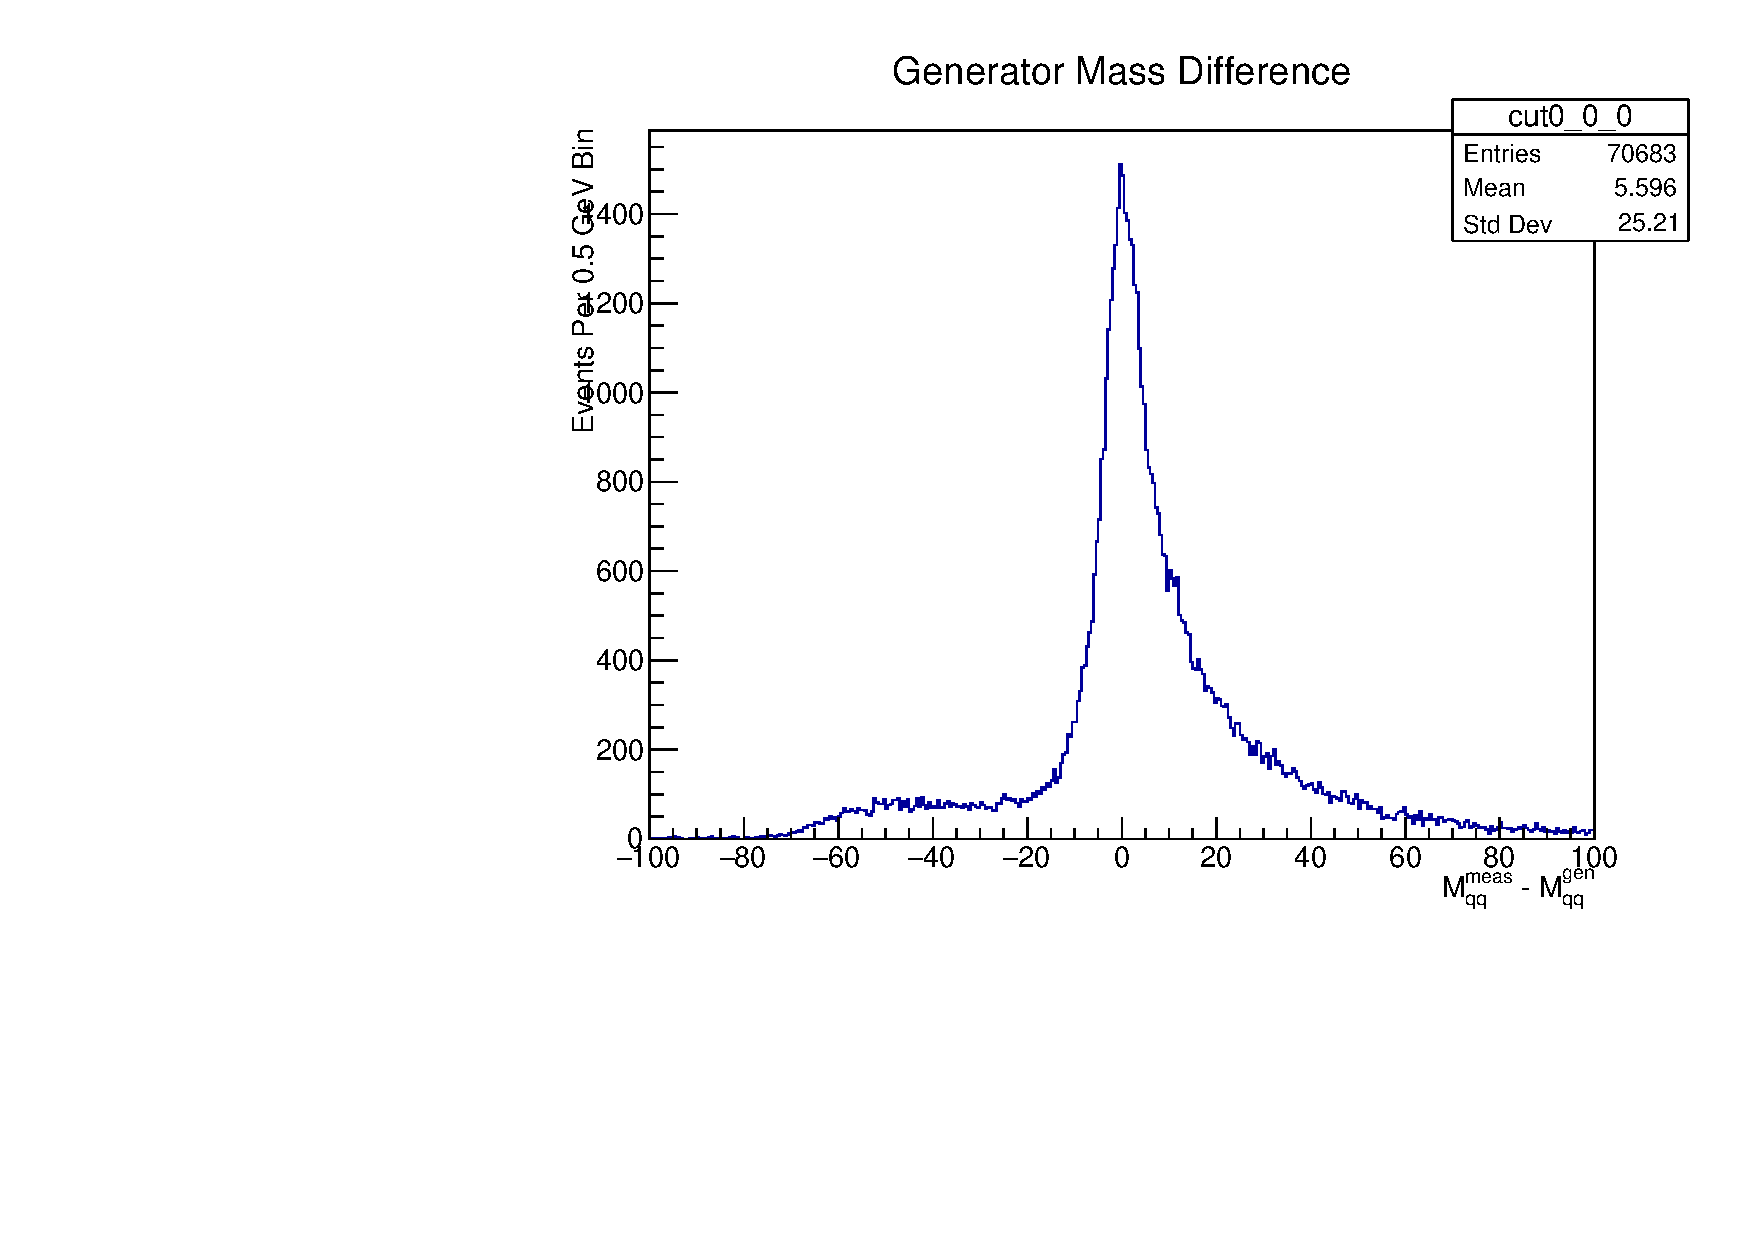
\includegraphics[scale=0.3]{nocutDiff.pdf}
\end{column}
\end{columns}


\end{frame}
\begin{frame}{(2) Optimized W Mass}
Find best W jet parameters over the ranges:\\
Use only signal events with gen. prompt muons\\
\begin{itemize}
\item[-]yCut:$[1\times10^{-3}, 5\times10^{-6}]$ \\
\item[-]pT:$[0,5]$ bins of 0.5 GeV\\
\item[-]$|cos\theta|$:$[0.9,1]$ 0.01 bins\\
\end{itemize}
\quad \quad \\
Use 2 optimization parameters from the $M_{qq}^{meas} - M_{qq}^{gen}$ dist.:\\
\begin{itemize}
\item[-] Full Width Half Maximum (FWHM) \\
\item[-]Number of bin Entries in the Mode\\
\end{itemize}
\quad \quad \\ 
\scriptsize
The Mode Entries is the number of entries in the Maximum bin + the number of Entries of the nearest left/right neighbor bins\\
The Mode is the weighted mean of the center of the 3 Mode bins\\
\quad \quad \\ 
The Maximum for the FWHM is the "Mode Average" or the average number of entries from the 3 mode bins\\
\quad \quad \\ 
The edges of the Width for FWHM are the weighted average between the 2 bins around the half maximum ( 1 bin above 1 bin below) 
\end{frame}

\begin{frame}{(2) Hadronic System Results}

\begin{columns}
\begin{column}{0.5\textwidth}
   	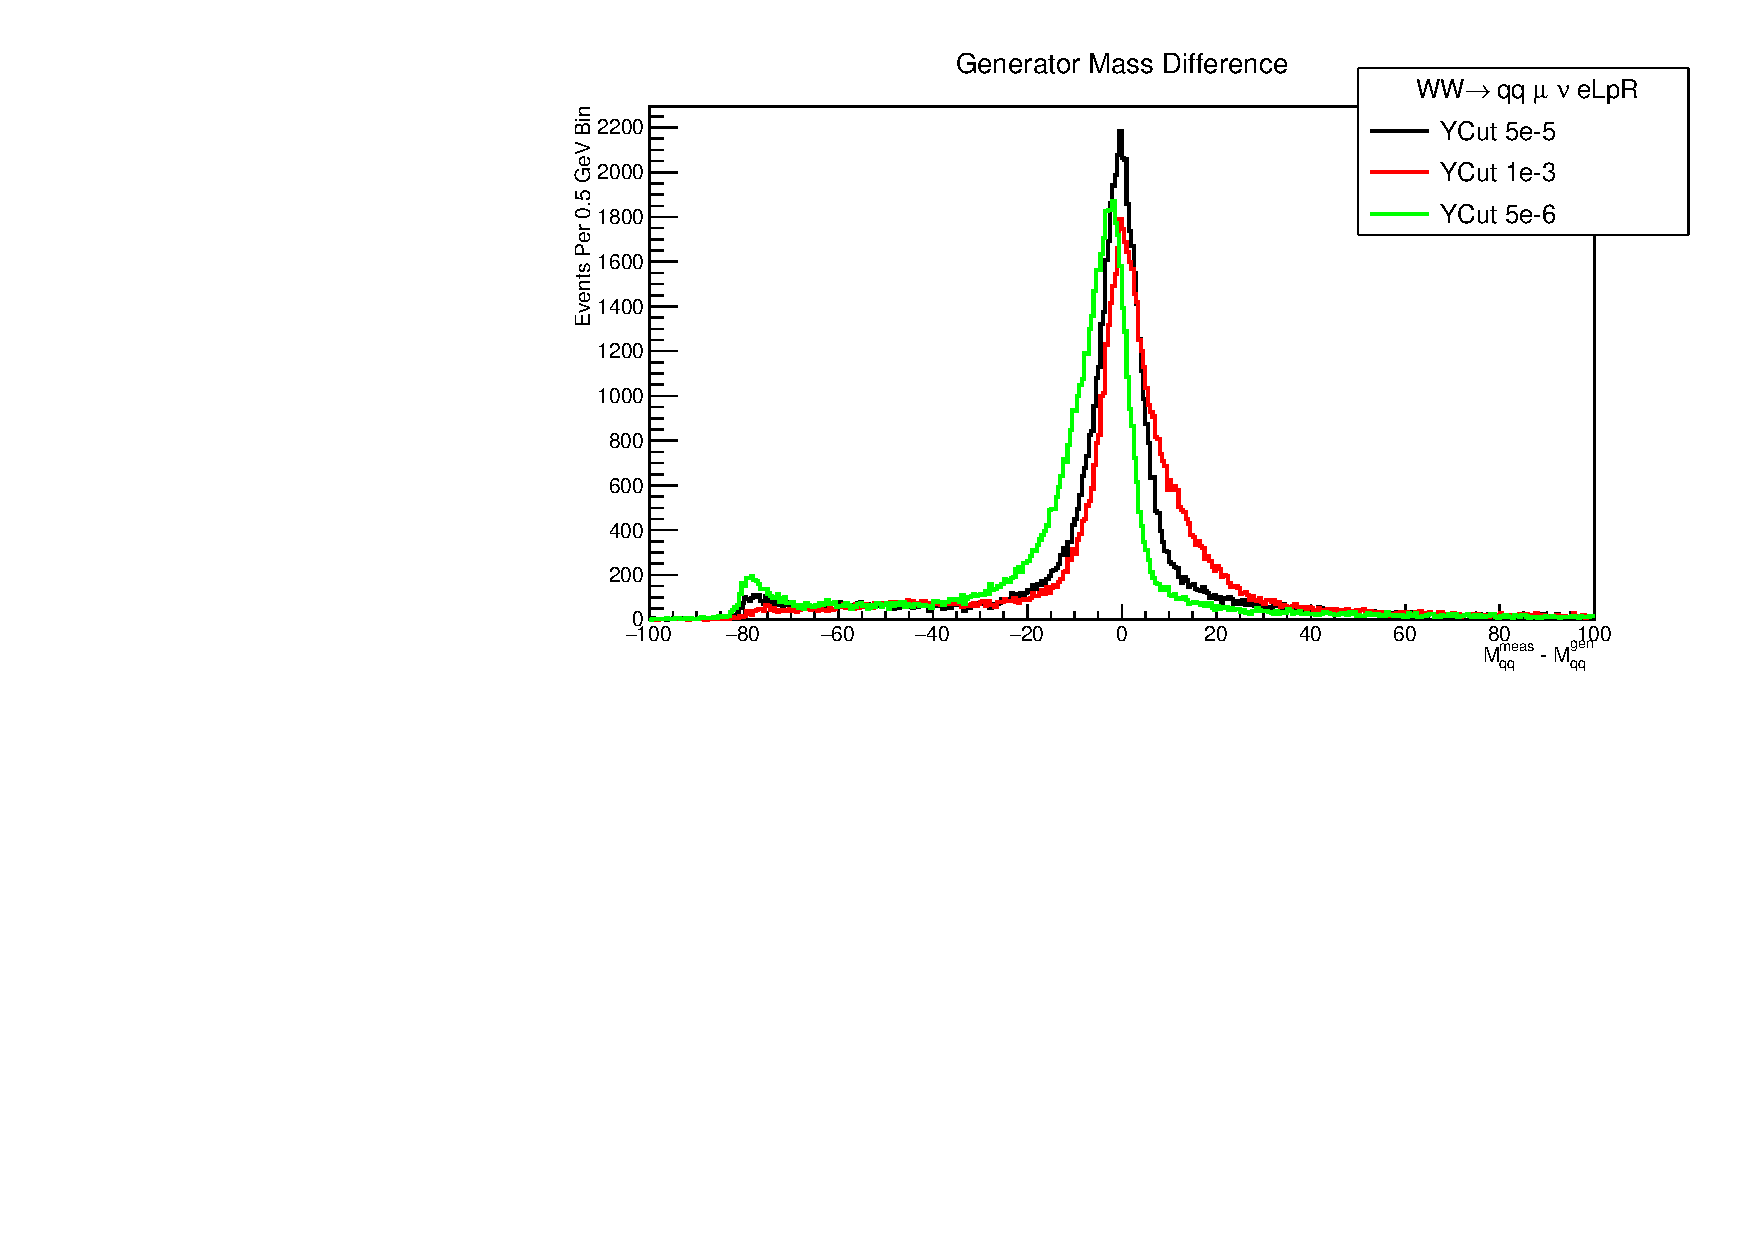
\includegraphics[scale=0.3, left]{SupDiff.pdf}\\
   	\scriptsize
   	Comparison of 3 YCuts with the same kinematic cuts Pt$>$2 GeV AND $|cos\theta|<$1 (optimized for 5e-05)\\
   	\quad \quad \\
   	Small peak around -80 GeV is where the W has been incorrectly thrown out\\
   	\quad \quad \\
   	
   
\end{column}
\begin{column}{0.5\textwidth}
	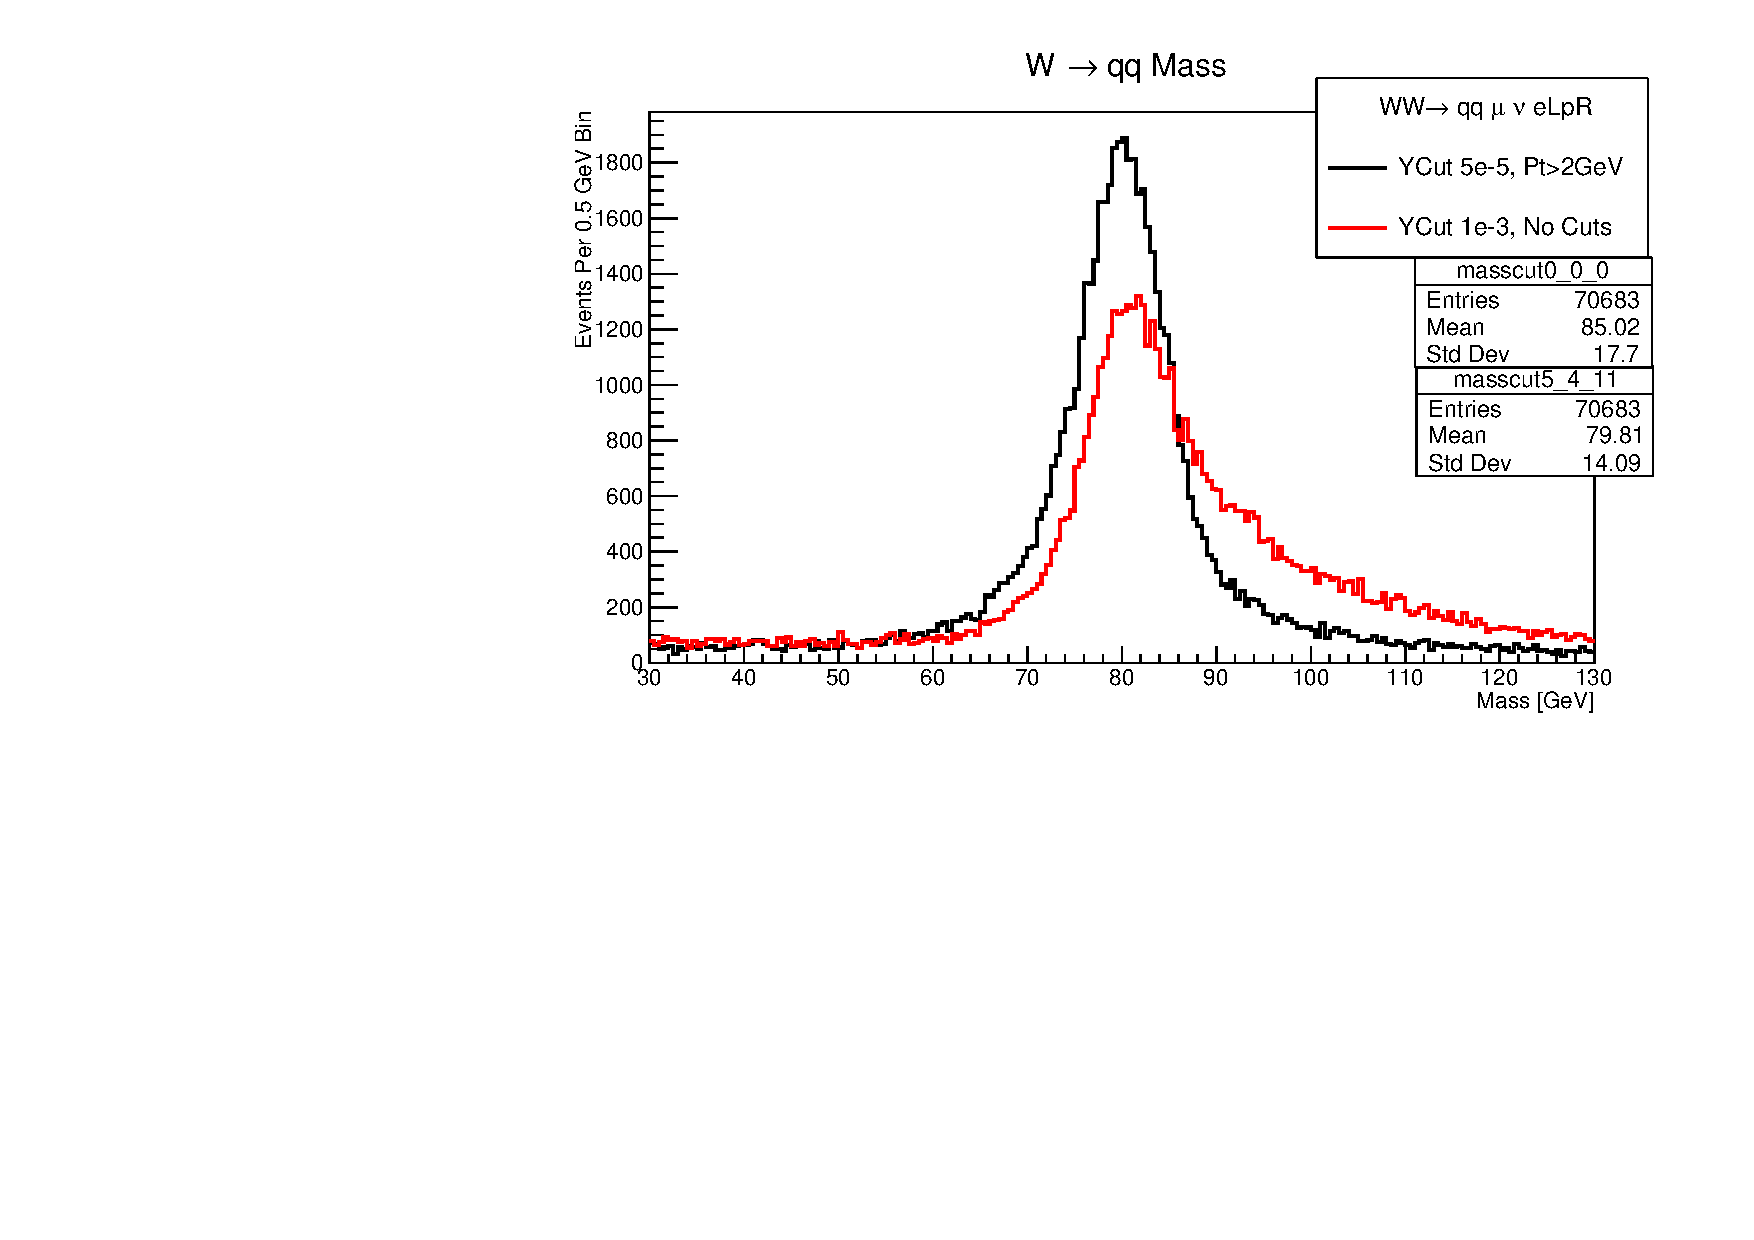
\includegraphics[scale=0.3, left]{SupMass.pdf}\\
	\scriptsize
	\quad \quad \quad \quad Significant Improvement !
\end{column}	
\end{columns}
\tiny
 Mass Difference Statistics:\\
 ycut: 0.001  ptcut: 2  costcut: 1  FWHM: 11.769 RMS: 24.1855 Mode: -0.24211 mean: 0.782898 modeEnt: 5199\\
 ycut: 5e-05  ptcut: 2  costcut: 1  FWHM: 9.7087 RMS: 25.2774 Mode: -0.25127 mean: -3.09776 modeEnt: 6326\\
 ycut: 5e-06  ptcut: 2  costcut: 1  FWHM: 11.567 RMS: 25.7475 Mode: -1.75521 mean: -9.57673 modeEnt: 5475\\

\quad \quad \\
\normalsize
Best Performance is reached with:\\
\textbf{ycut= 5e-05 and removal of mini-jets with pT $<$ 2 GeV }


\end{frame}
\begin{frame}{(3) Event Selection Overview}
Perform event selection with two mutually exclusive groups:\\
1st group will use $\mu$ cone (optimized for prompt muons)
	\begin{itemize}
		\scriptsize
		\item[-]``tight" selection will yield some efficiency $\epsilon_0$ and purity $p_0$
		\item[-] tight cuts will be targeted towards prompt signal leptons $\mu/e$ 
	\end{itemize} 
2nd group will use the $\tau$ cone (optimized for inclusive $\tau$ decays)
	\begin{itemize}
	\scriptsize
		\item[-] ``loose" selection will yield some efficiency $\epsilon_1$ and purity $p_1$
		\item[-] ``loose" cuts should address $\tau$s not reconstructed by muon cone
		\item[-] orthognalize selection require 0 tight leptons in loose selection
	\end{itemize}
Optimize selection for some overall efficiency $\epsilon = \epsilon_0 + \epsilon_1$ times purity $p = (N_0 + N_1) / (B_0 + B_1 + N_0 +N_1)$\\
\quad \quad \\
Description of current cuts:(currently tight/loose are mostly the same)\\
\tiny
adapted from ref. \url{I. Marchesini DESY-THESIS 2011}\\
\scriptsize
--Note reconstucted particles are boosted against crossing angle boost-- (3.5 GeV in x)\\
\begin{itemize}
\item[-]Lepton - Require at least 1 reconstructed lepton
\item[-]Track Multiplicity $> 10$ - at least 10 tracks in the event (targeting rejection of 2f Bkg.)
\item[-]Pt $> 5$ GeV - reject events with no genuine missing Pt 
\item[-]$E_{vis} < 500$ GeV Sum of the total visible energy in the event 
\item[-]$E_{com} > 100$ GeV - target rejection of 2f and leptonic eeZ, $E_{com} = E_{vis} + |P_{miss}| \, \,  \, \, P^\mu_{miss} = (|P_{miss}| , -\sum{\vec{p}_{vis}}) $
\item[-]$40<M_{qq}<120$ - constrains jet system to be W-like
\item[-] $-qcos\theta_W$ - require the $W^-$ to scatter forward

\end{itemize}


	
	

\end{frame}

\begin{frame}{(3) Event Selection (Tight)}
\scriptsize
Tight Signal $\Rightarrow$  muon cone for $\mu,e,\tau$ signal events\\
All plots include an N Lepton $> 0$ cut (except N Lepton plot)\\
Polarization: (-0.8,+0.3)\quad
Luminosity: 1600 fb$^{-1}$
\begin{columns}
\begin{column}{0.5\textwidth}
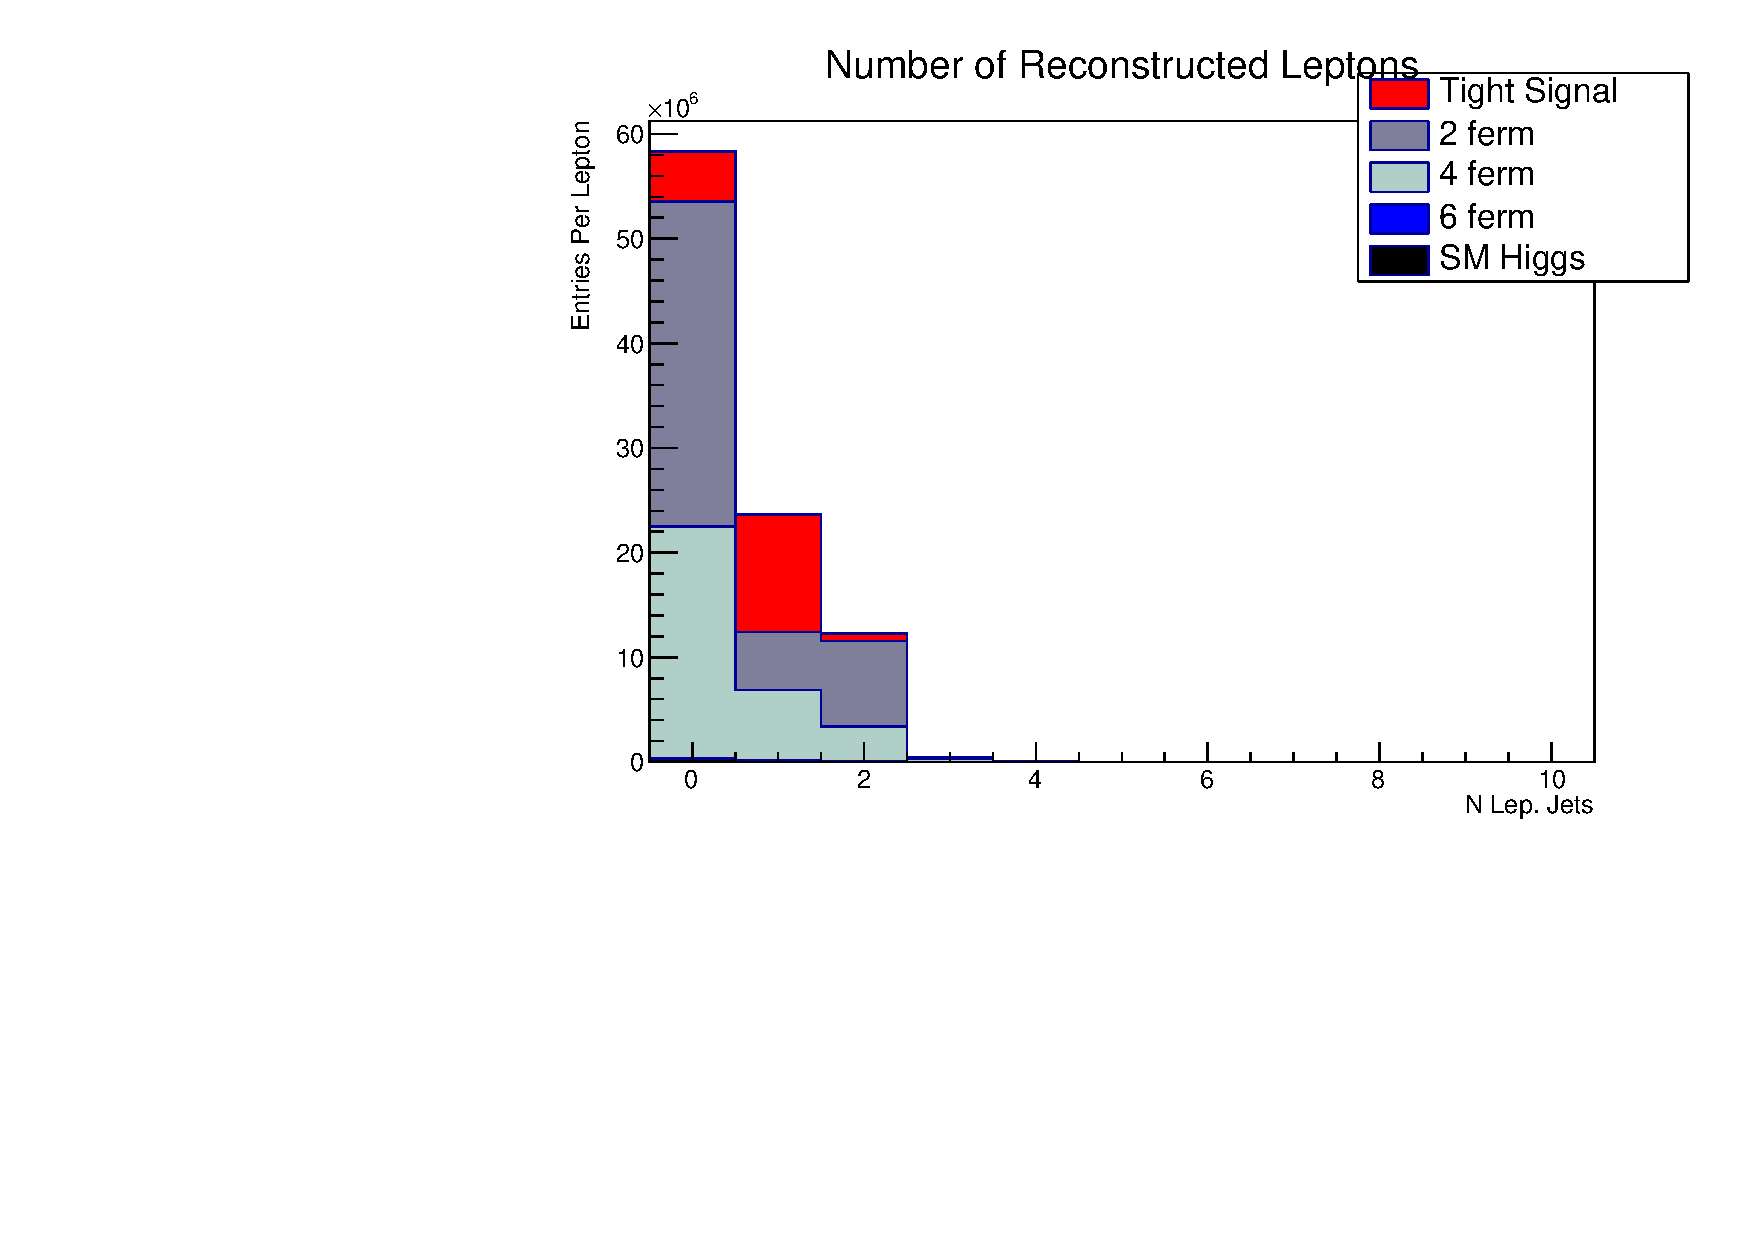
\includegraphics[scale=0.3, left]{nLepHist.pdf} \\
N Leptons $> 0$
\end{column}
\begin{column}{0.5\textwidth}
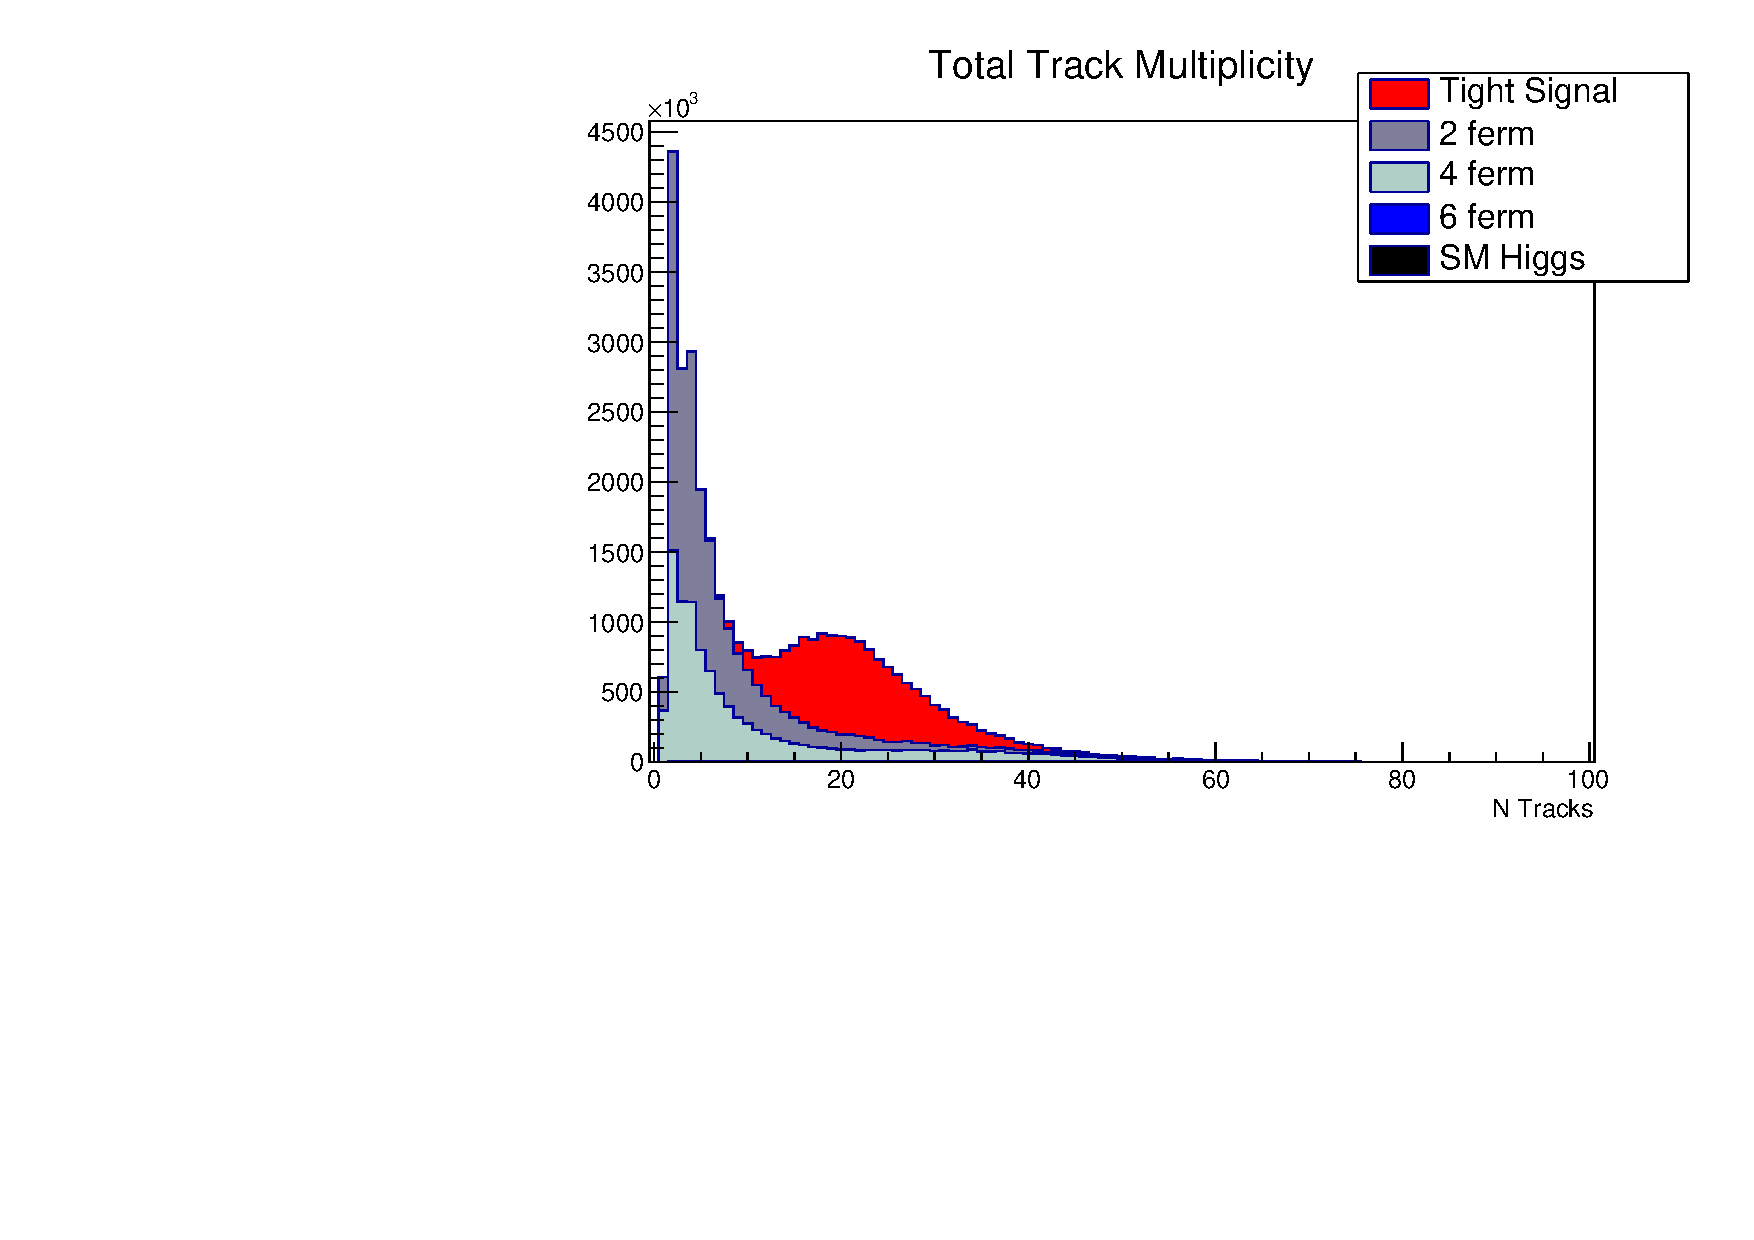
\includegraphics[scale=0.3, left]{ntracksHist.pdf} \\
N Tracks $> 10$
\end{column}
\end{columns}
\end{frame}

\begin{frame}{(3) Event Selection (Tight)}
\scriptsize
Tight Signal $\Rightarrow$  muon cone for $\mu,e,\tau$ signal events\\
All plots include an N Lepton $> 0$ cut\\
Polarization: (-0.8,+0.3)\quad
Luminosity: 1600 fb$^{-1}$
\begin{columns}
\begin{column}{0.5\textwidth}
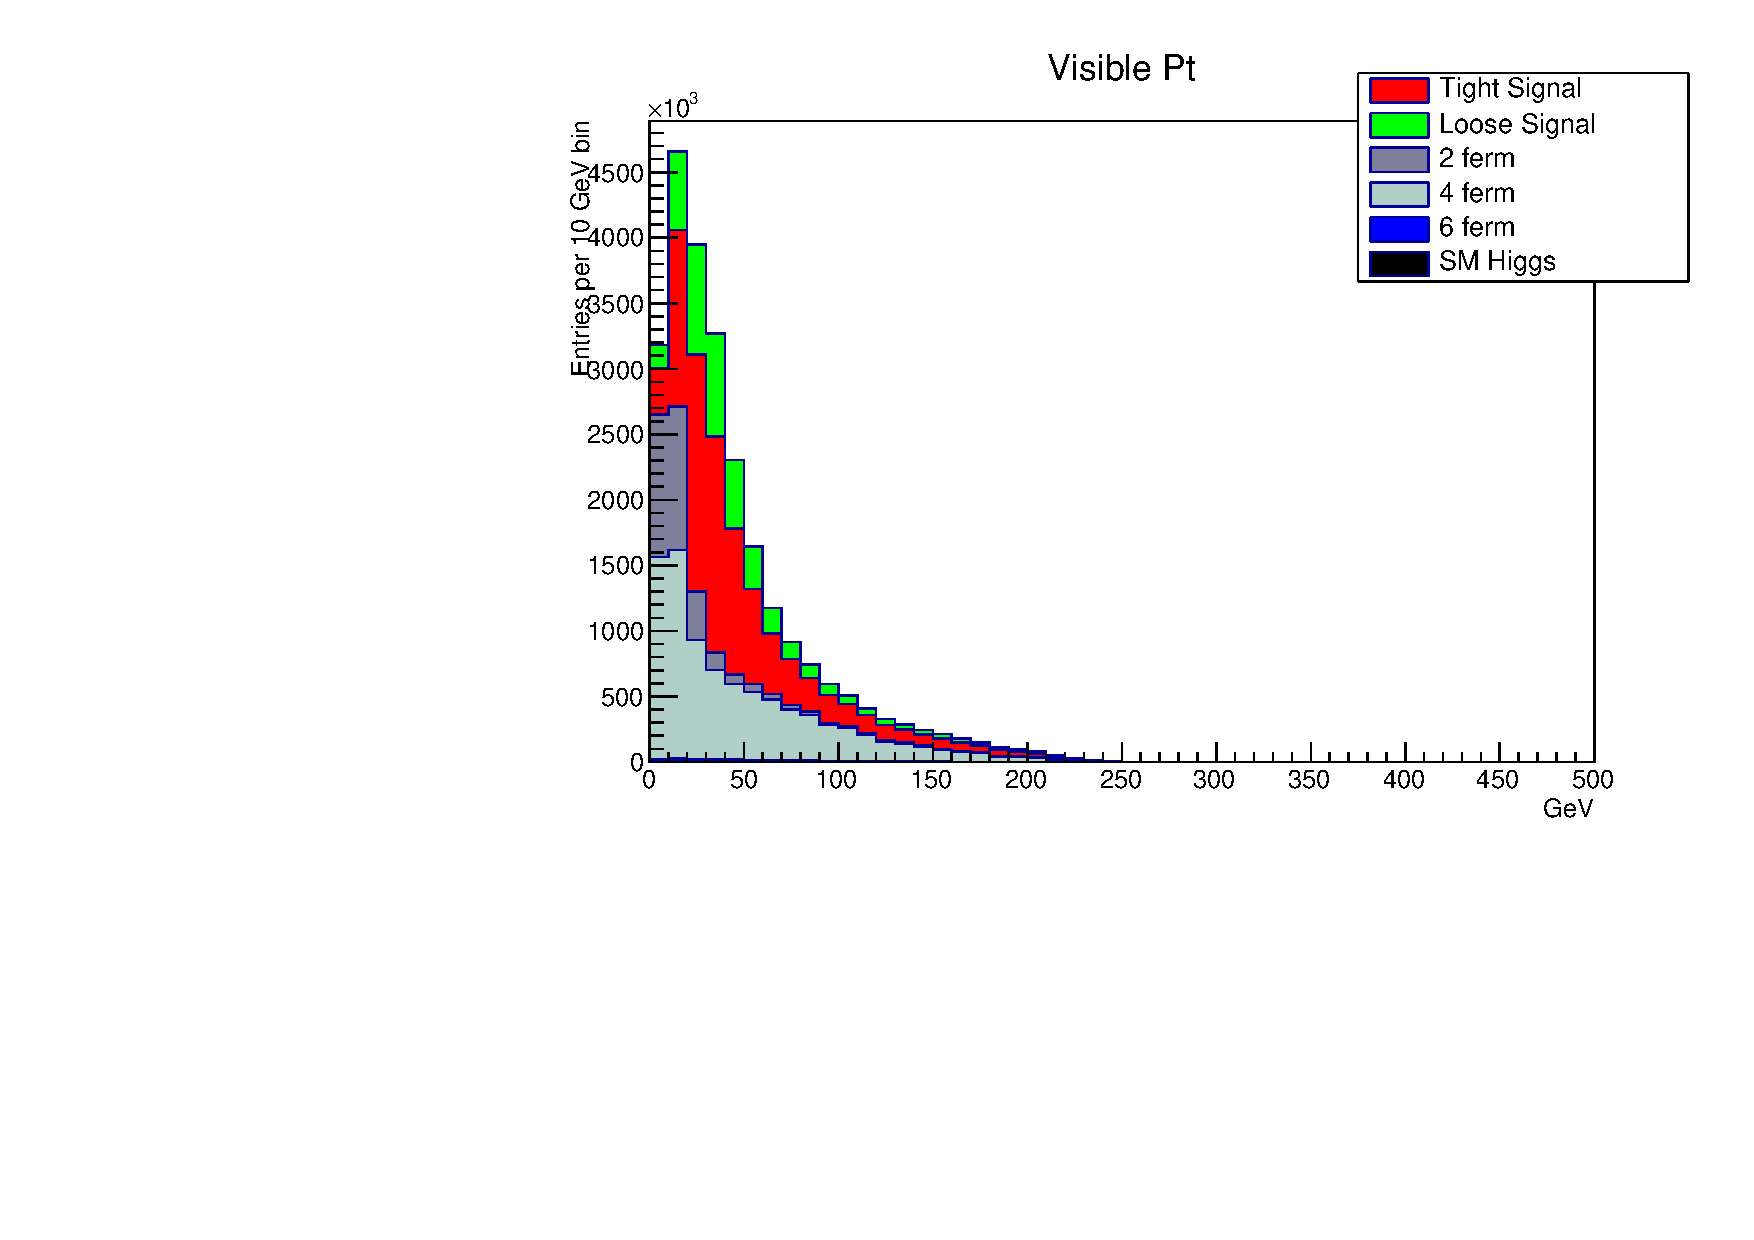
\includegraphics[scale=0.3, left]{PtvisHist.pdf} \\
Visible Pt $> 5$ GeV
\end{column}
\begin{column}{0.5\textwidth}
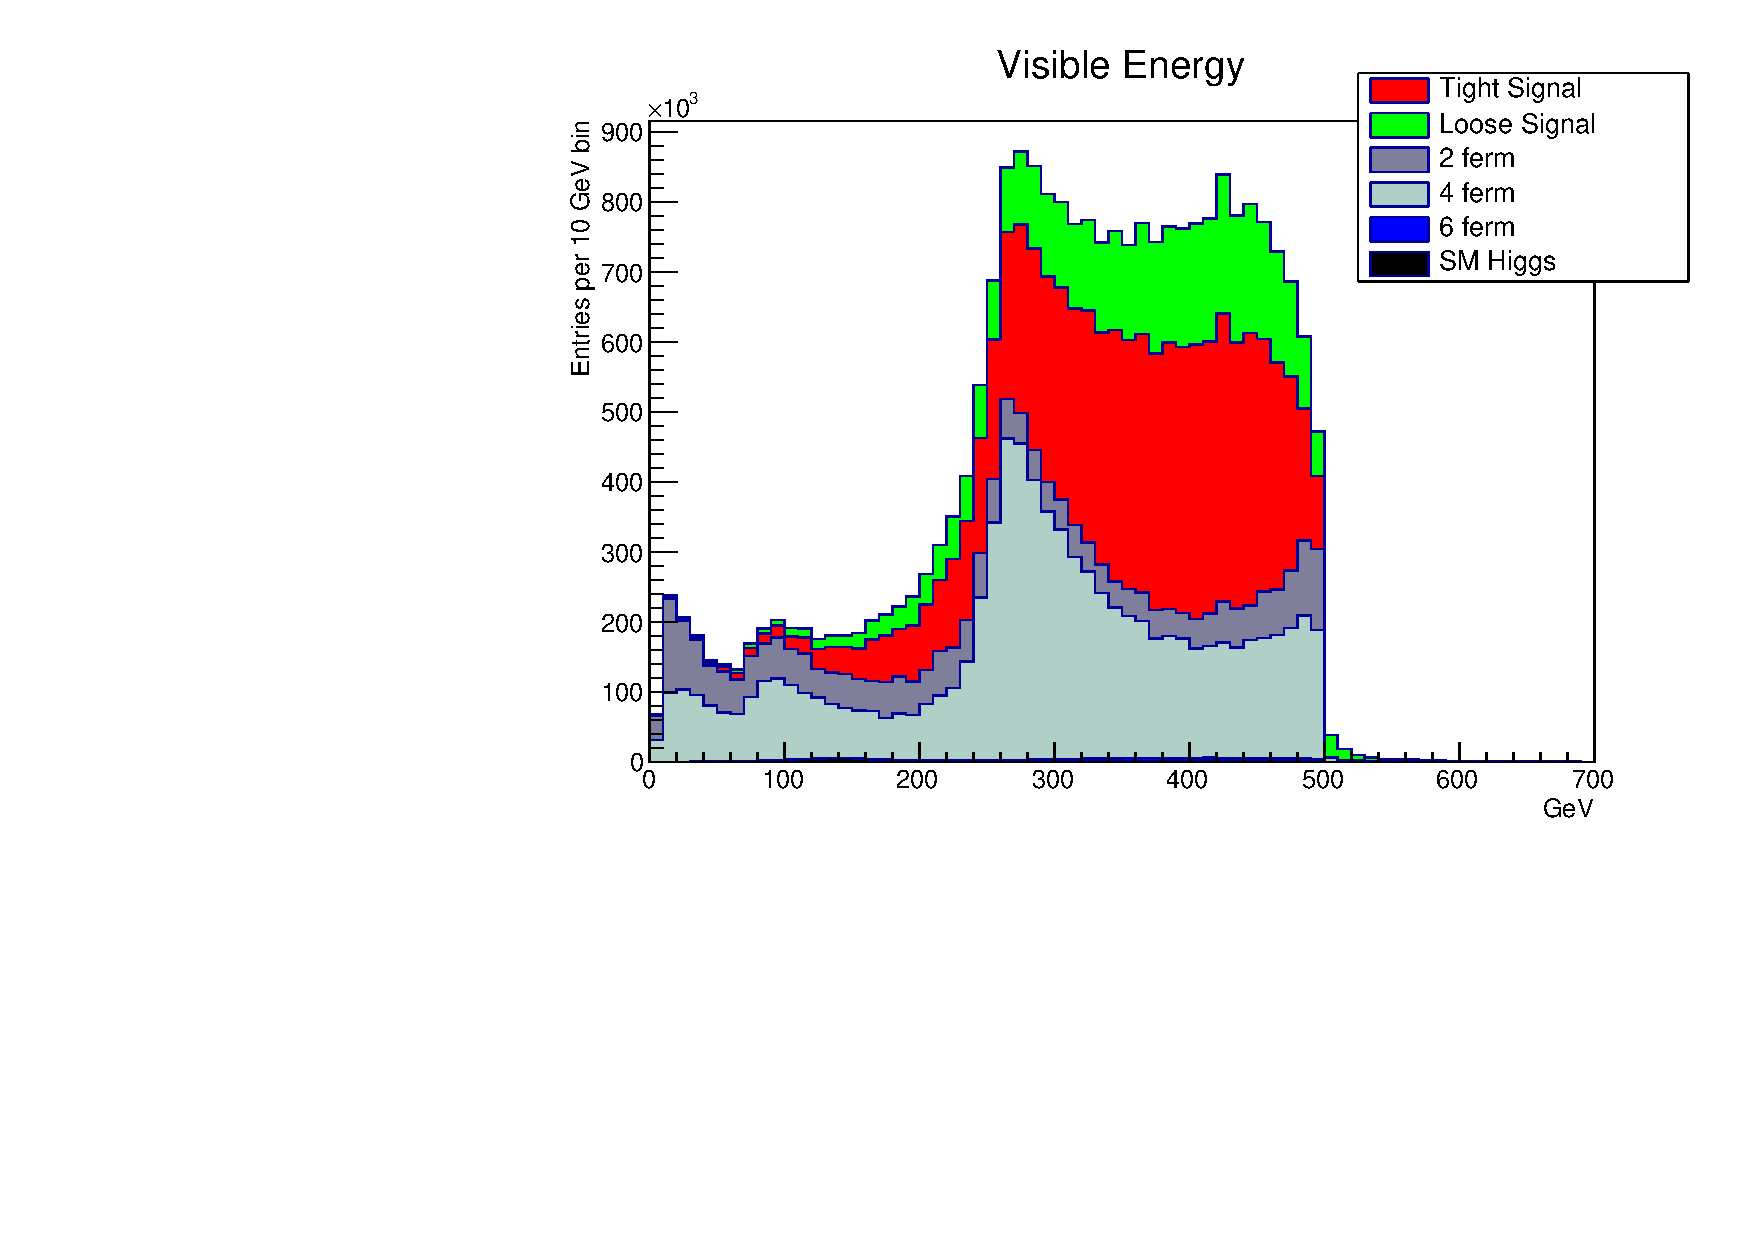
\includegraphics[scale=0.3, left]{EvisHist.pdf} \\
Visible Energy $< 500$ GeV
\end{column}
\end{columns}
\end{frame}

\begin{frame}{(3) Event Selection (Tight)}
\scriptsize
Tight Signal $\Rightarrow$  muon cone for $\mu,e,\tau$ signal events\\
All plots include an N Lepton $> 0$ cut\\
Polarization: (-0.8,+0.3)\quad
Luminosity: 1600 fb$^{-1}$
\begin{columns}
\begin{column}{0.5\textwidth}
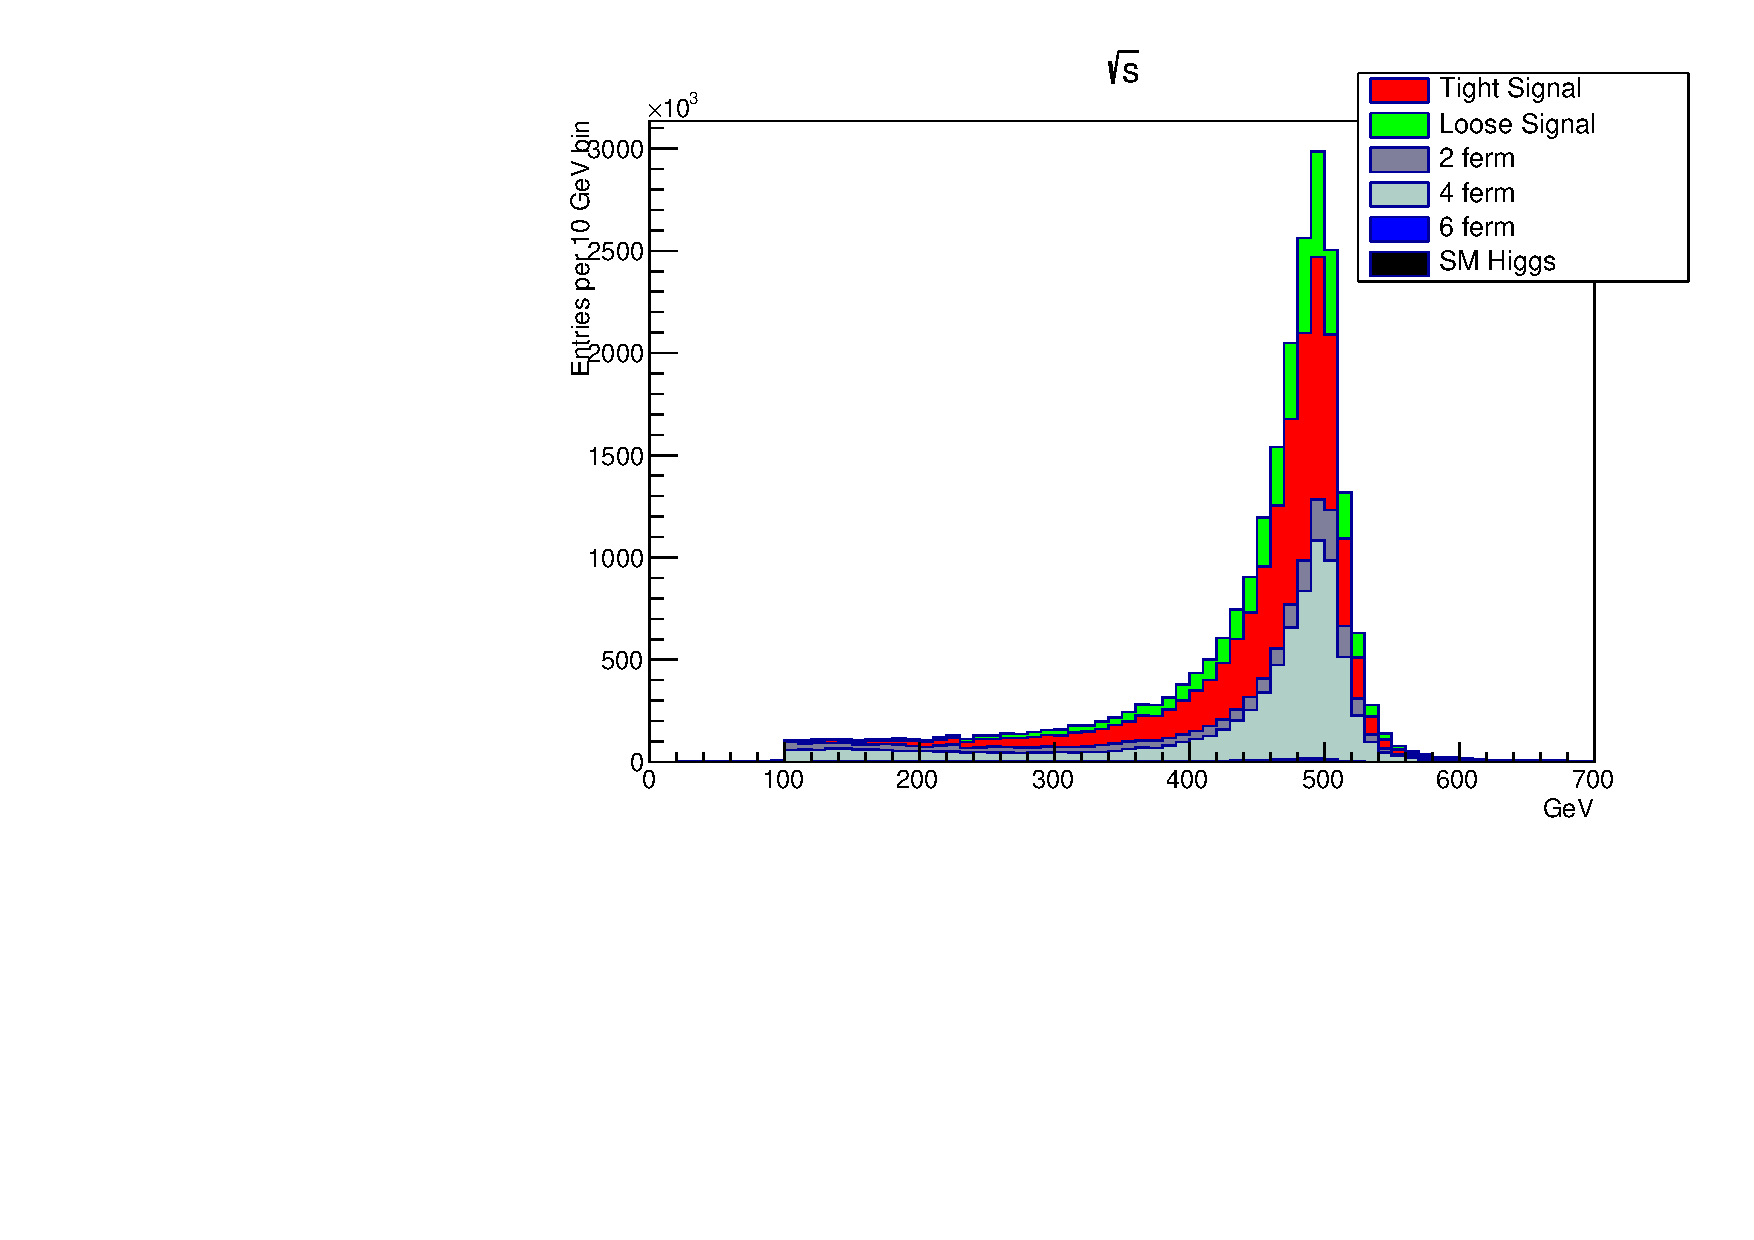
\includegraphics[scale=0.3, left]{EcomHist.pdf} \\
$E_{com} > 100$ GeV
\end{column}
\begin{column}{0.5\textwidth}
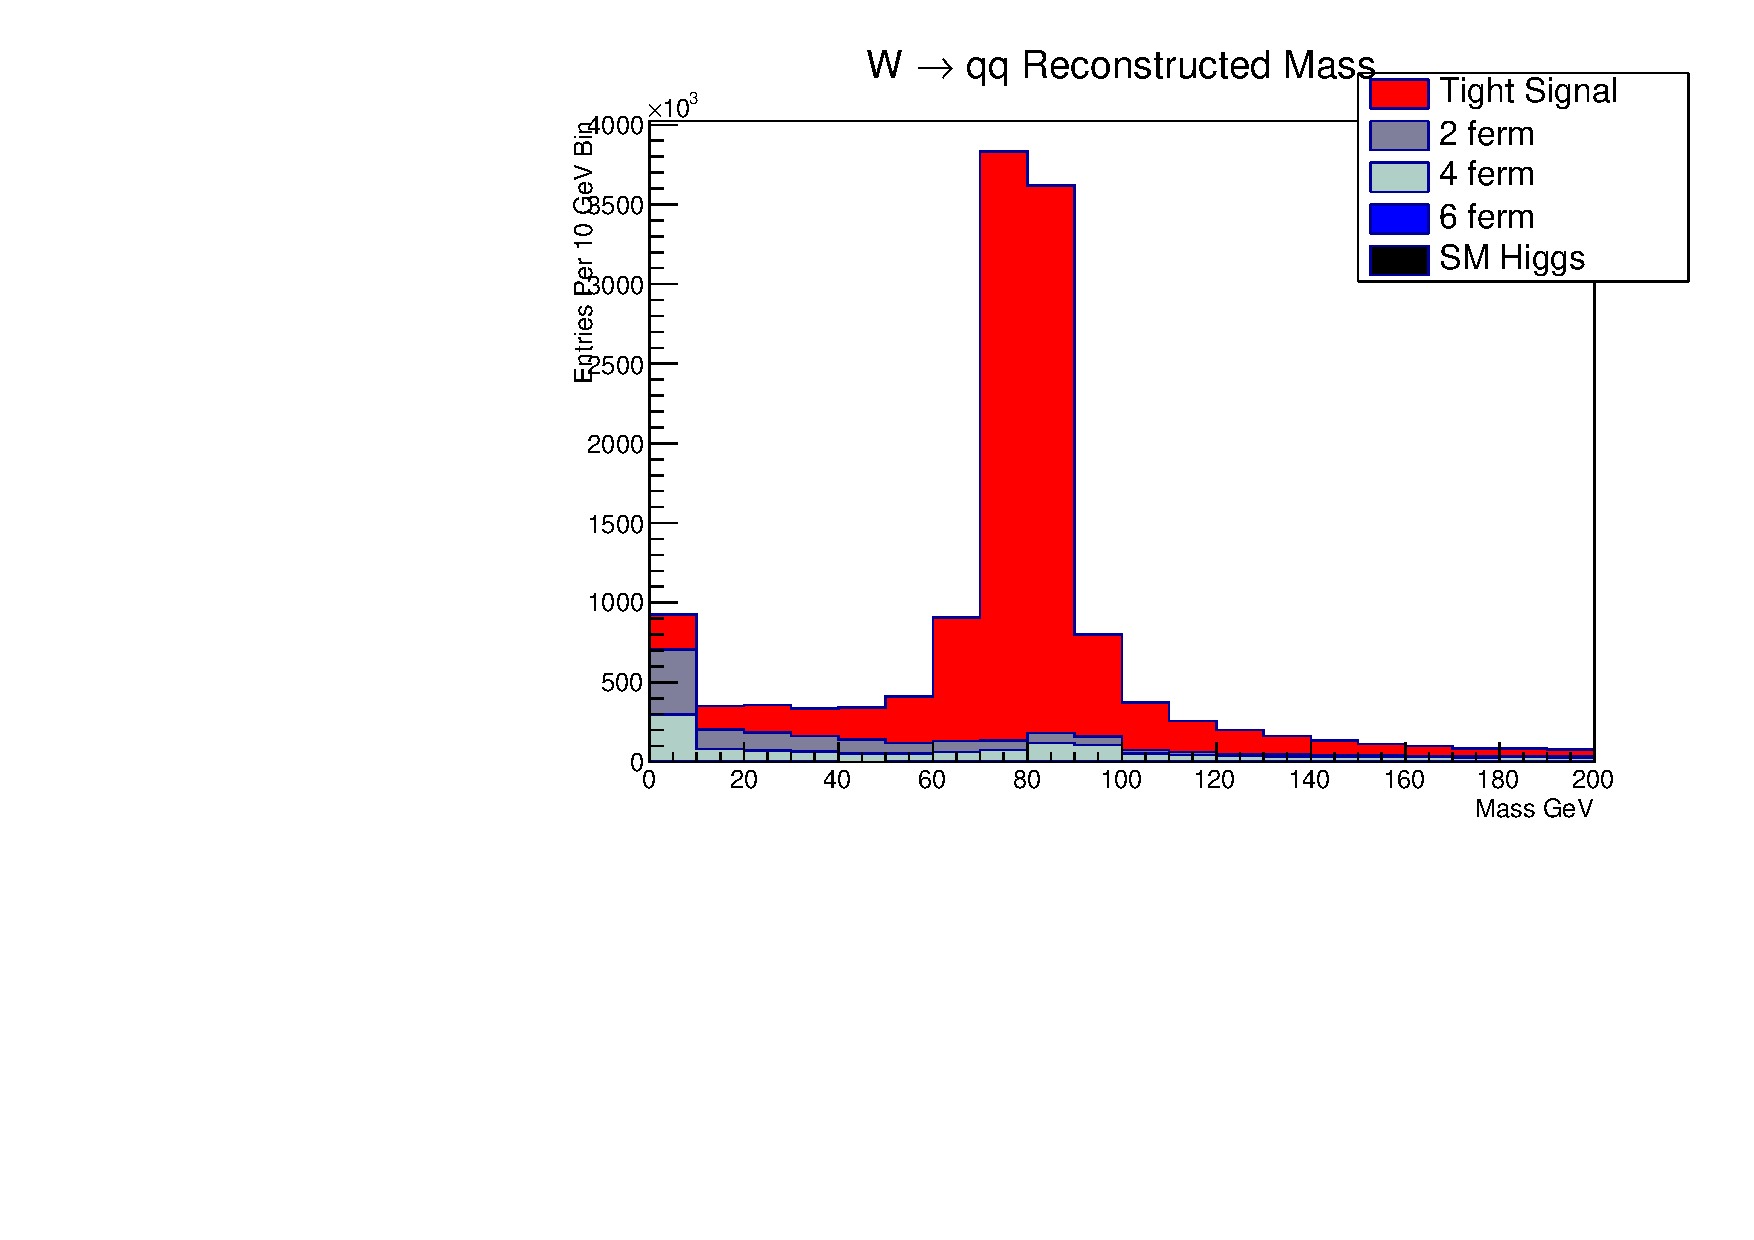
\includegraphics[scale=0.3, left]{mwhadHist.pdf} \\
$ 40 < M_{qq} < 120$
\end{column}
\end{columns}
\end{frame}

\begin{frame}{(3) Event Selection (Tight)}
\scriptsize
Tight Signal $\Rightarrow$  muon cone for $\mu,e,\tau$ signal events\\
All plots include an N Lepton $> 0$ cut\\
Polarization: (-0.8,+0.3)\quad
Luminosity: 1600 fb$^{-1}$\\
\begin{columns}
\begin{column}{0.5\textwidth}
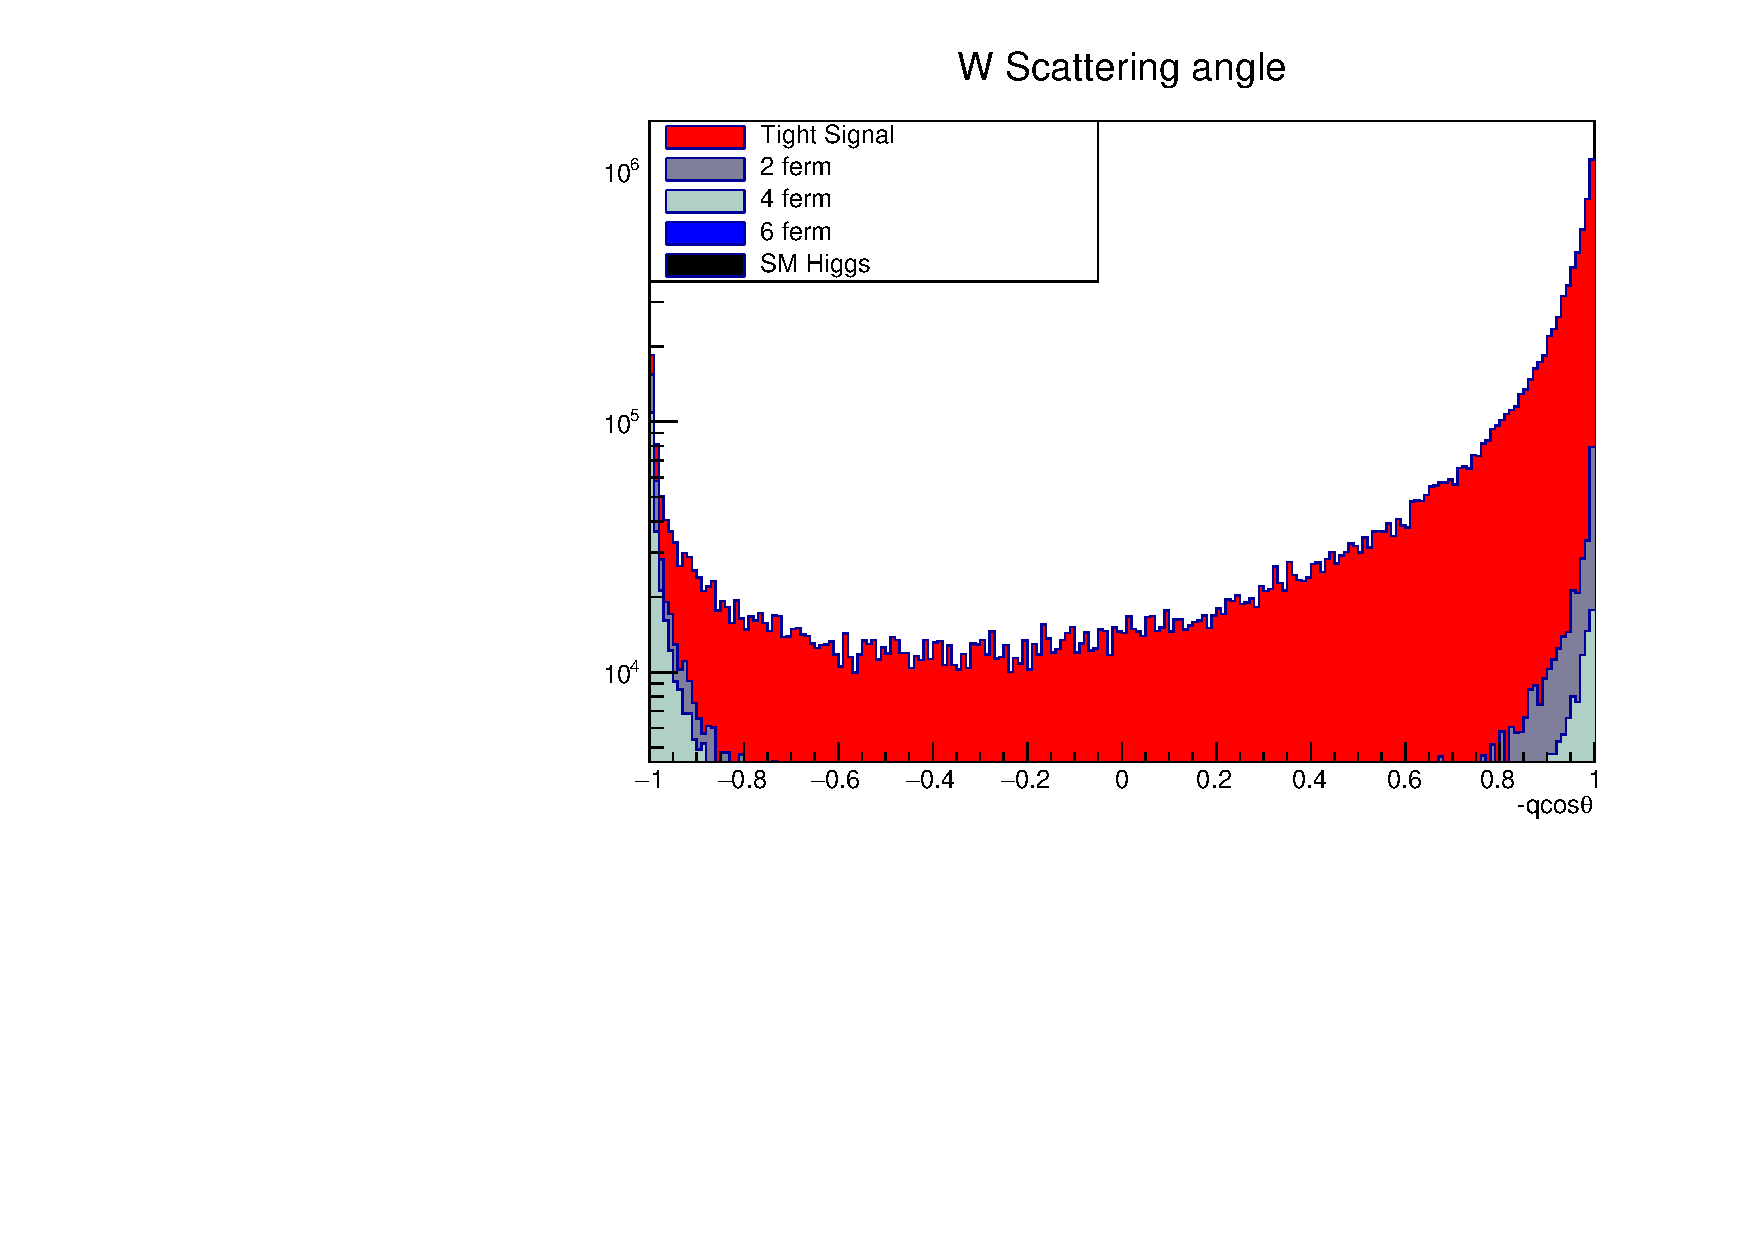
\includegraphics[scale=0.3, left]{qcostHist.pdf} \\
$-qcos\theta_W > -0.95$
\end{column}
\begin{column}{0.5\textwidth}

\end{column}
\end{columns}
\end{frame}
\begin{frame}{(3) Event Selection (Tight)}
Performance of hadronic mass and $W^{-}$ scattering angle\\
Polarization: (-0.8,+0.3)\quad
Luminosity: 1600 fb$^{-1}$\\
All cuts applied, tight selection only with $\mu ,e, \tau$

\begin{columns}
\begin{column}{0.5\textwidth}
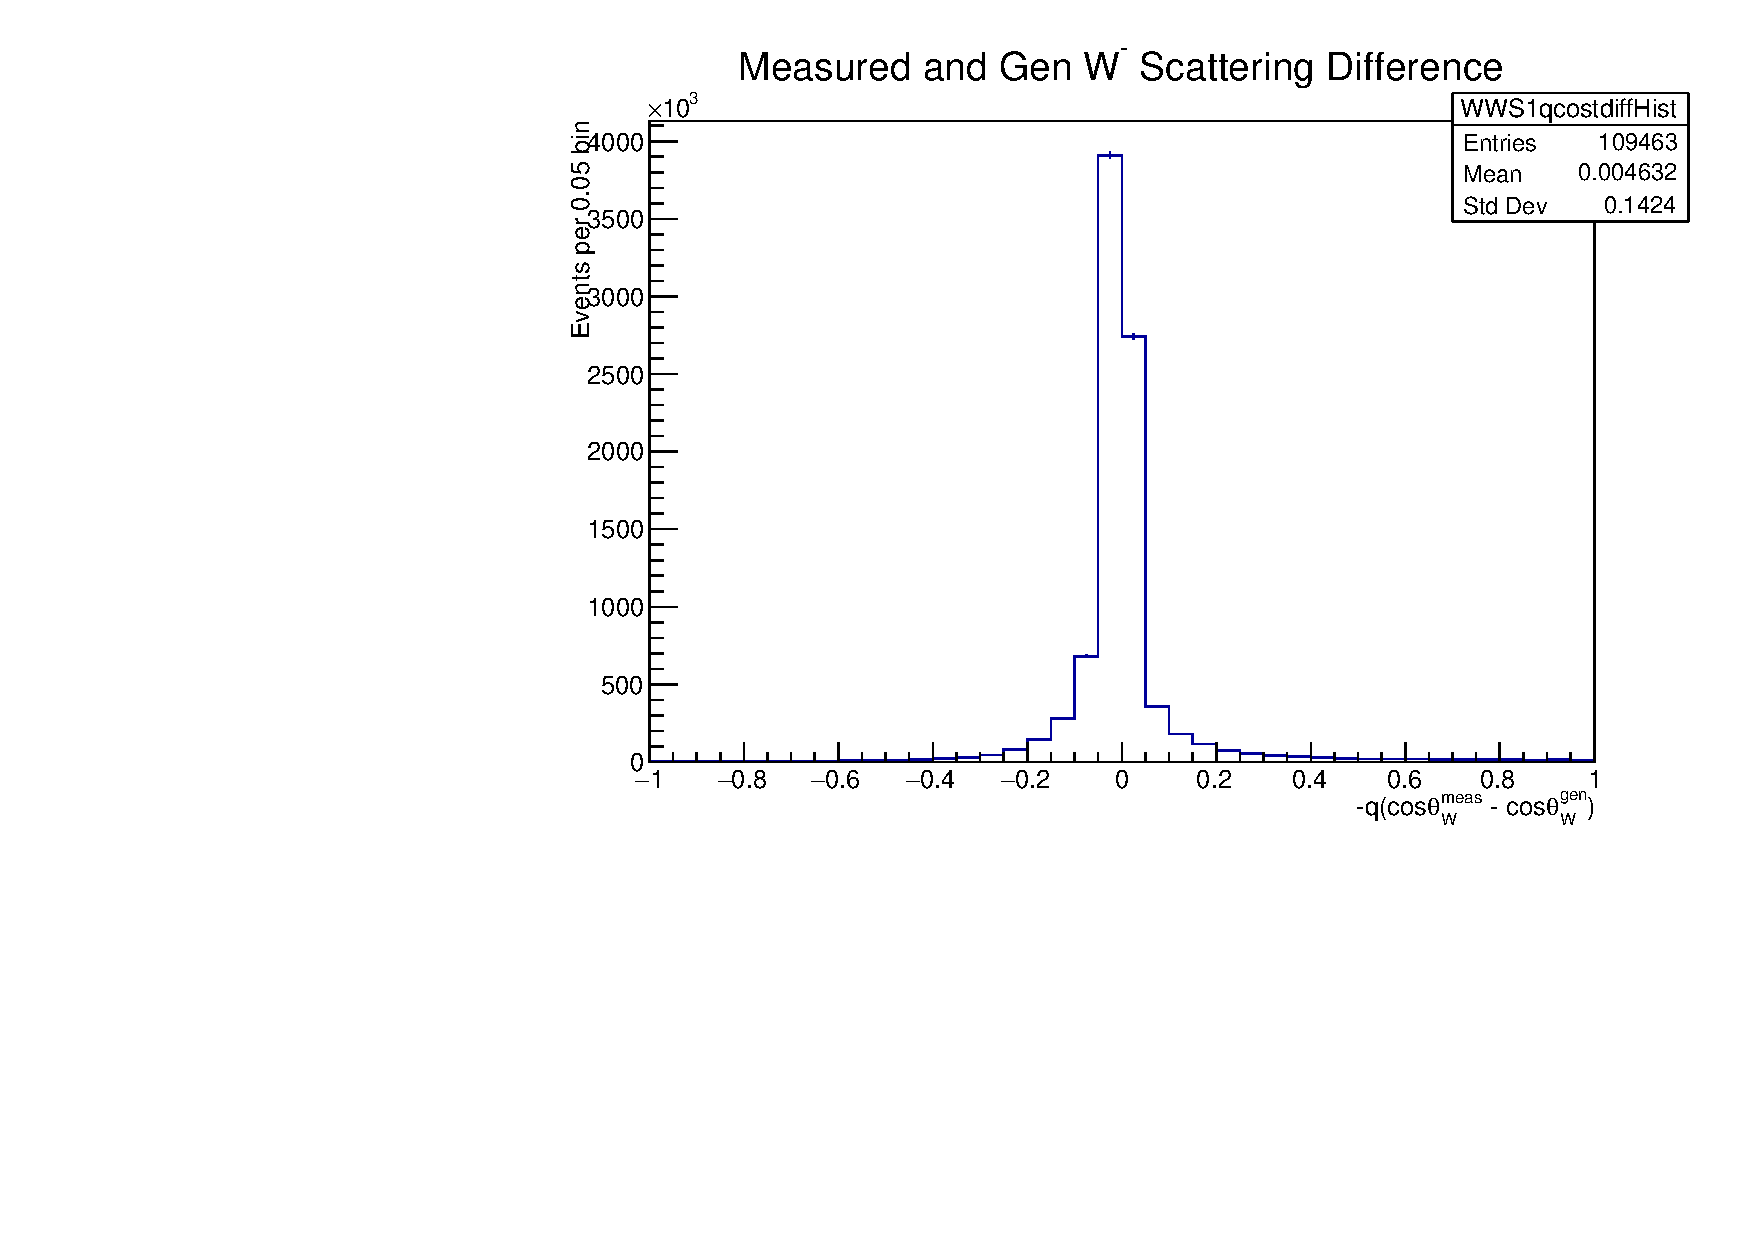
\includegraphics[scale=0.3, left]{qcostdiffHist.pdf} \\

\end{column}
\begin{column}{0.5\textwidth}
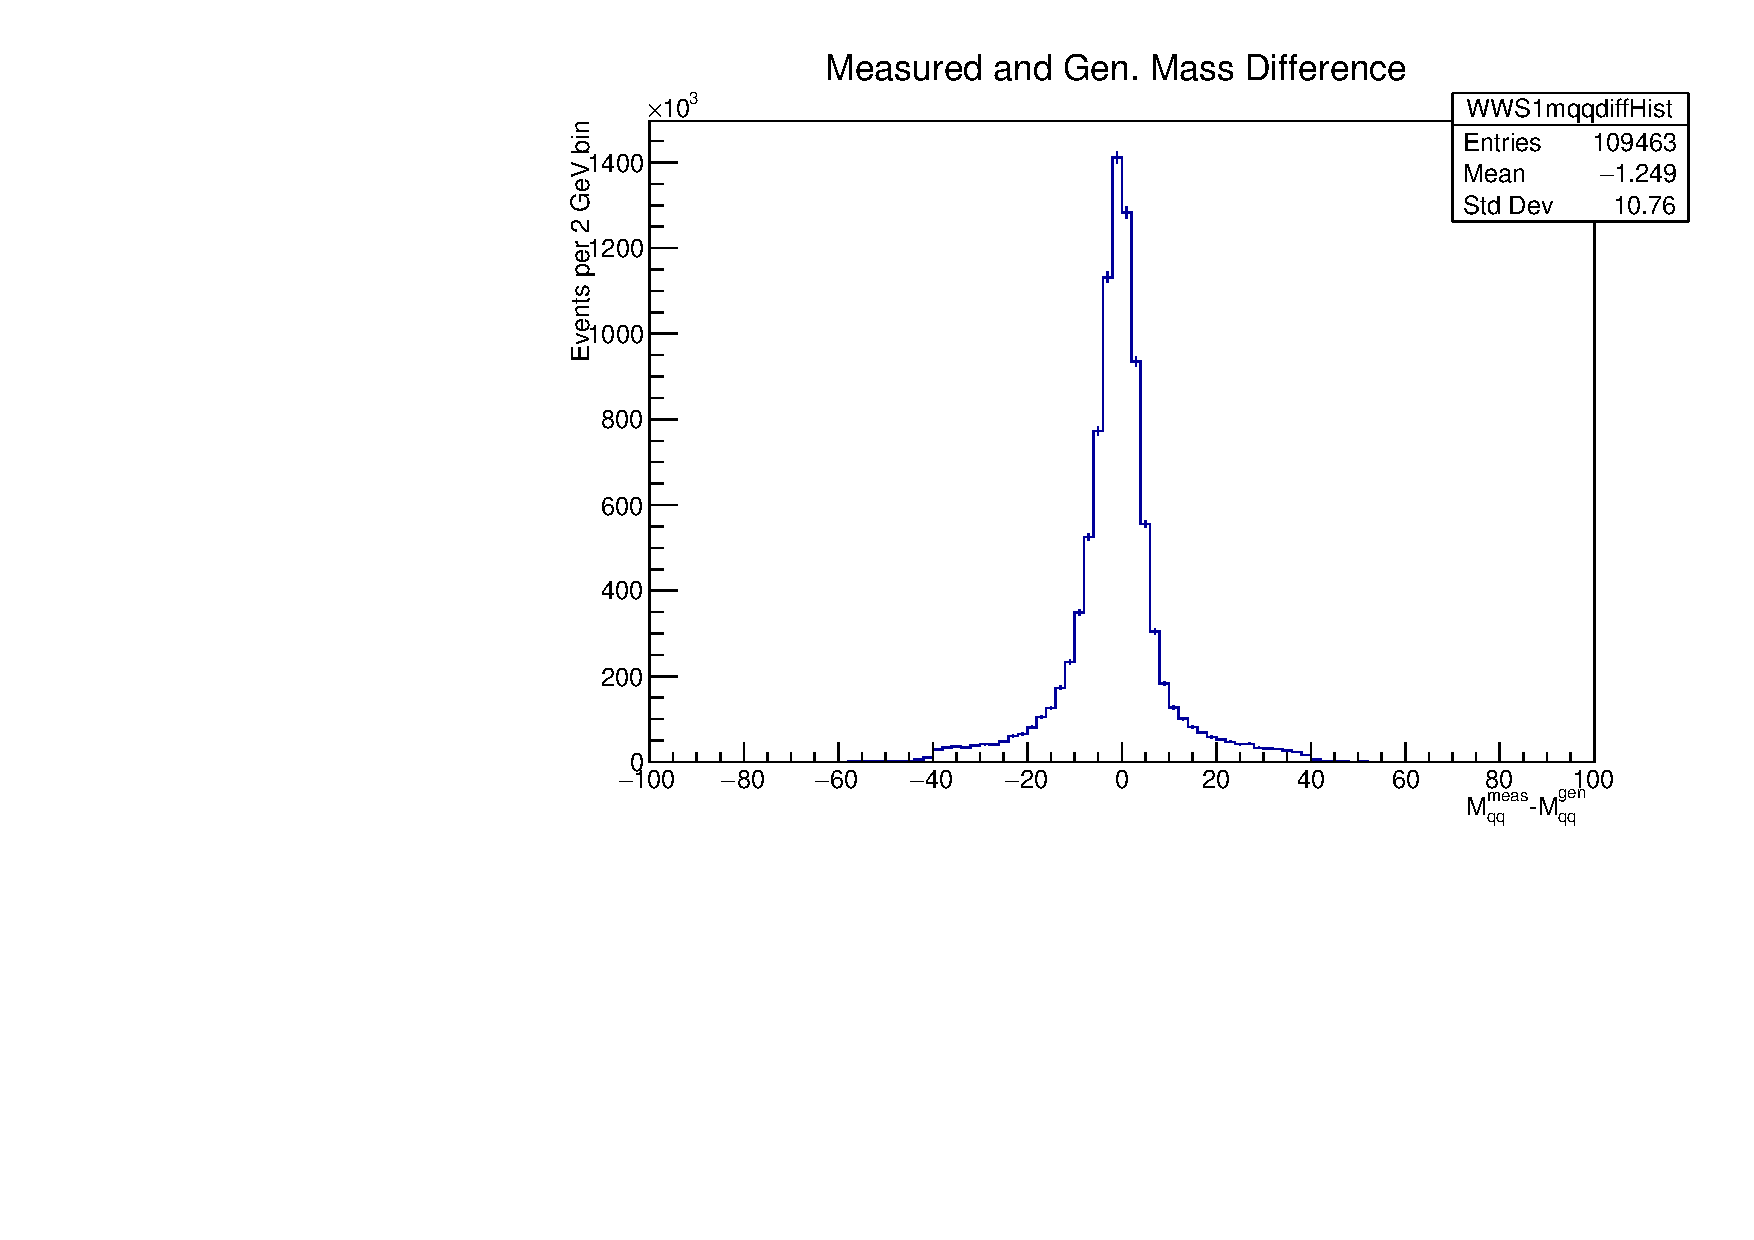
\includegraphics[scale=0.3, left]{mqqdiffHist.pdf} \\

\end{column}
\end{columns}

\end{frame}
\begin{frame}
Comparison of Generator mass differences\\
with pileup rejection and selection cuts vs. no pileup rejection or selection cuts
\scriptsize
\begin{columns}
\begin{column}{0.5\textwidth}
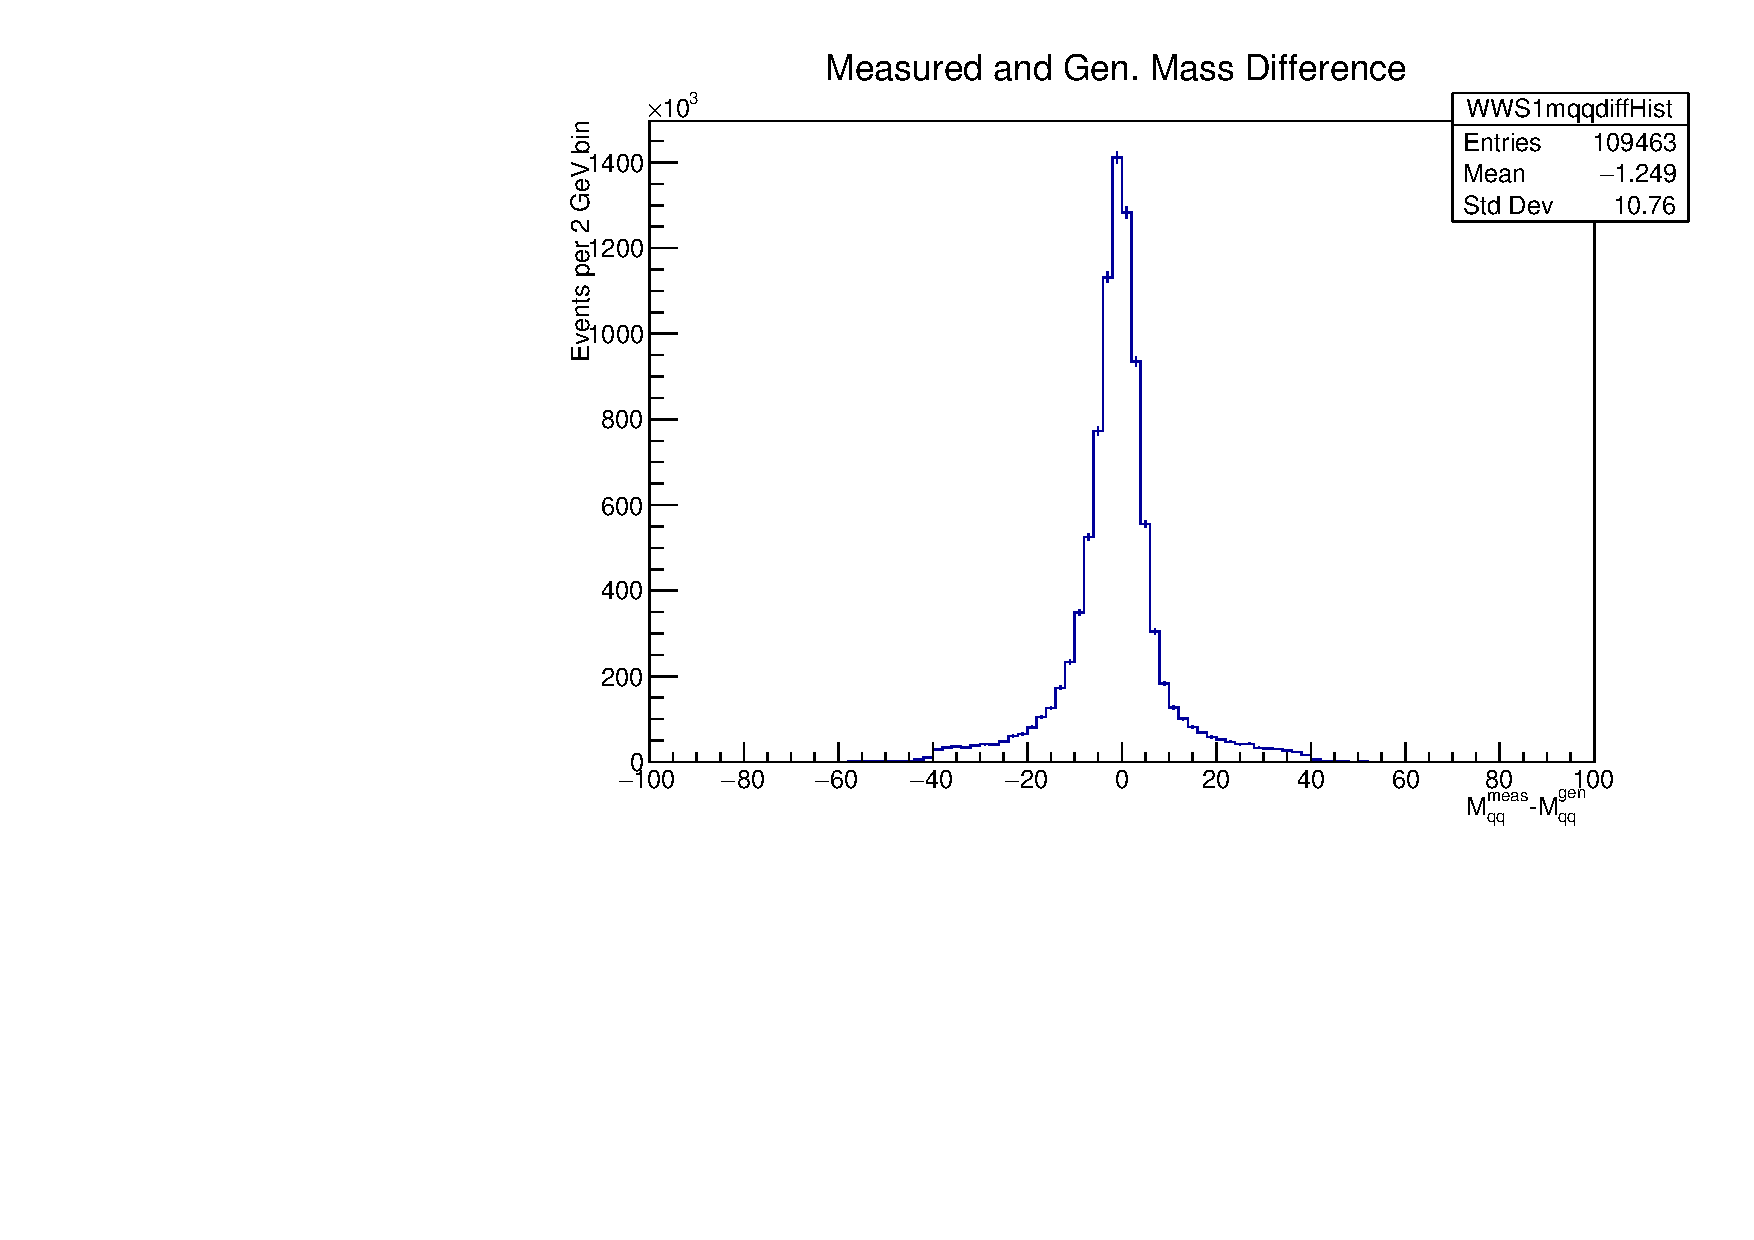
\includegraphics[scale=0.3, left]{mqqdiffHist.pdf} \\
 after cuts
\end{column}
\begin{column}{0.5\textwidth}
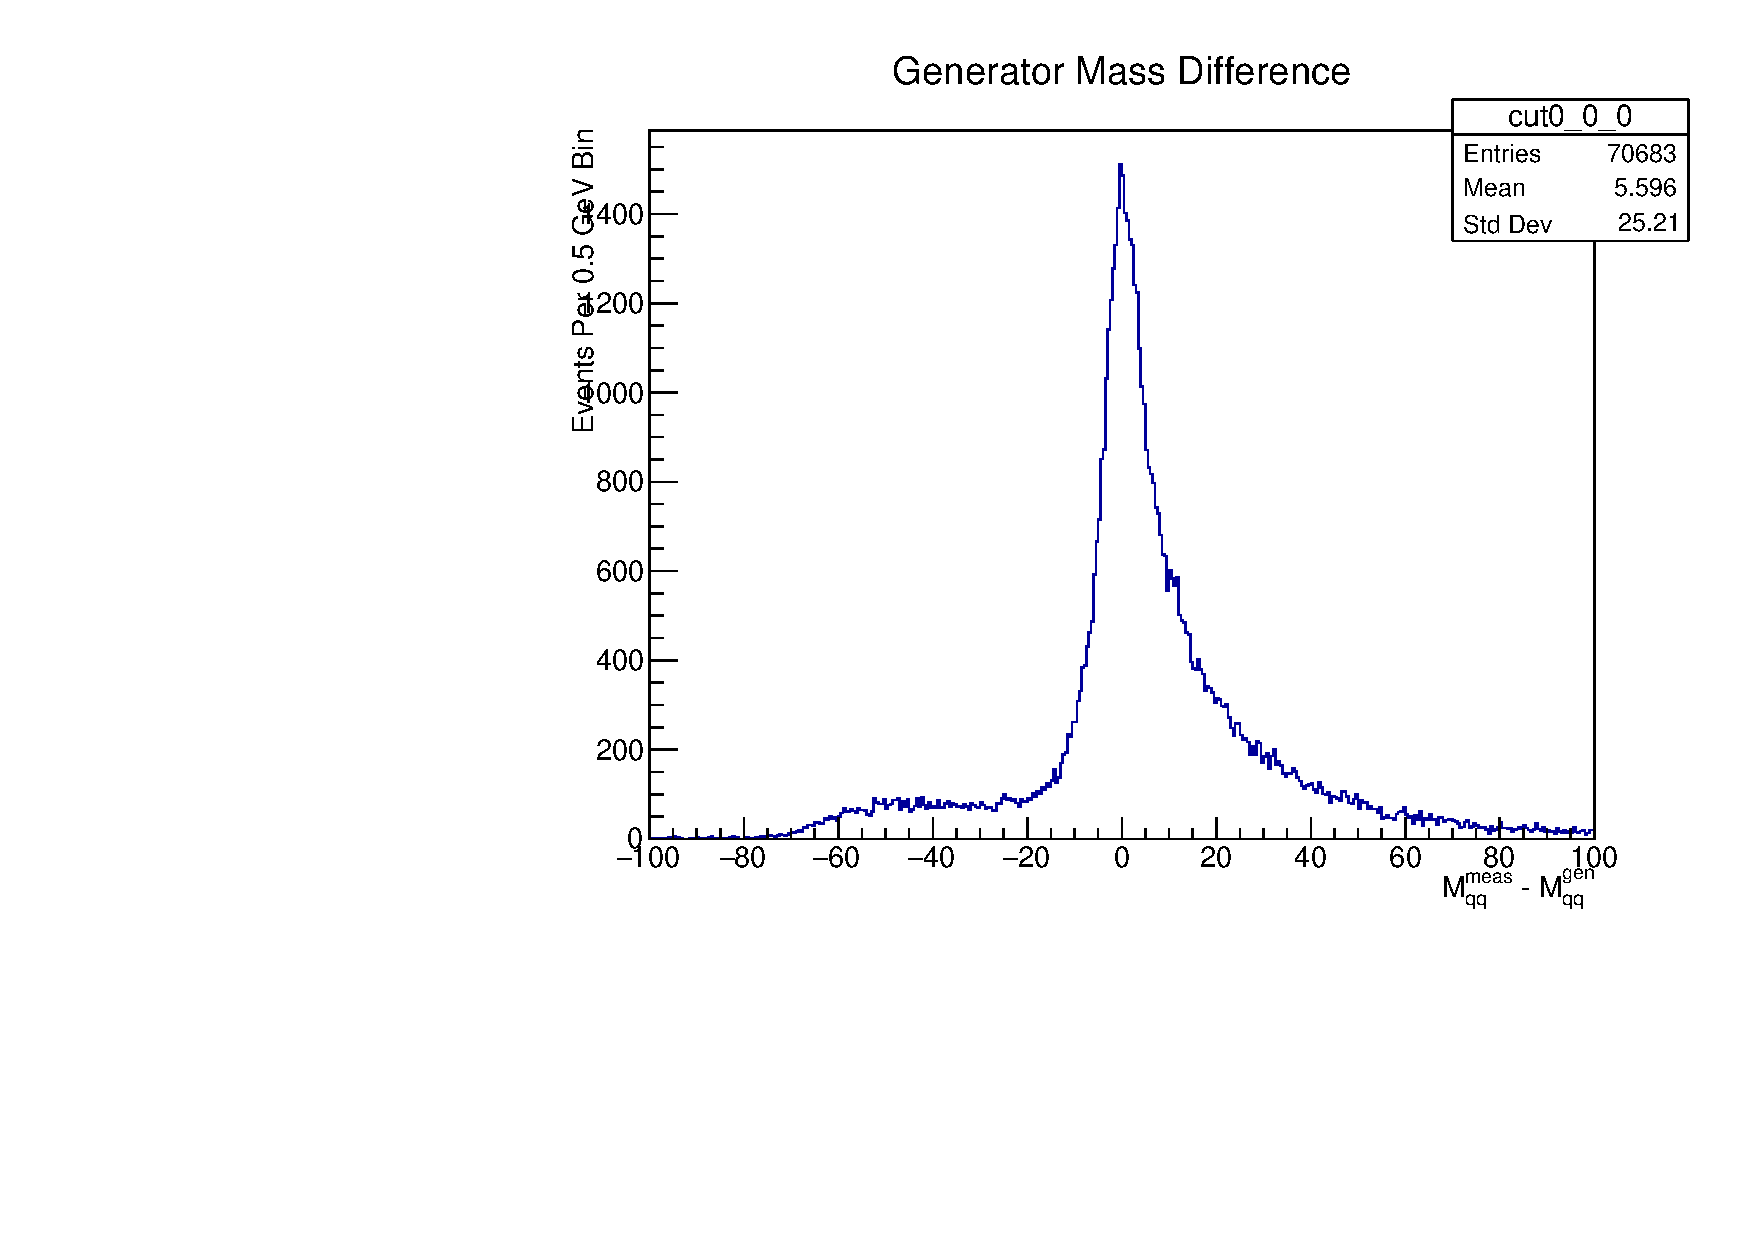
\includegraphics[scale=0.28, left]{nocutDiff.pdf} \\
before cuts
\end{column}
\end{columns}
\quad \quad \\
\quad \quad \\
Note: right distribution is not weighted and $100\%$ LR

\end{frame}

\begin{frame}{(3) Event Selection -- ``WW-like" Signal}
\scriptsize
Polarization: (-0.8,+0.3)\quad
Luminosity: 1600 fb$^{-1}$
\makebox[\linewidth]{\parbox{12.5cm}{  %}}
\tiny
Tight Selection with muon cone\\
   \begin{tabular}{|p{0.08\textwidth}p{0.08\textwidth}p{0.08\textwidth}p{0.08\textwidth}p{0.08\textwidth}p{0.08\textwidth}p{0.08\textwidth}p{0.08\textwidth}p{0.08\textwidth}|}
\hline 
   & Prompt $\mu$ & Prompt $e$ & $\tau$ & Tot. Sig. & 2f & 4f & 6f & Higgs \\ \hline 
Base Evts. &\num{3.87e+06 } & \num{3.89e+06 } & \num{3.90e+06} &\num{1.17e+07} & \num{4.22e+07} & \num{3.22e+07} & \num{2.14e+05} & \num{4.12e+05} \\ 
 
Lepton &\num{3.31e+06 } & \num{3.20e+06 } & \num{2.28e+06} &\num{8.78e+06} & \num{1.15e+07} & \num{1.18e+07} & \num{1.63e+05} & \num{1.15e+05} \\ 

N Tracks &\num{3.22e+06 } & \num{3.11e+06 } & \num{2.21e+06} &\num{8.54e+06} & \num{2.84e+06} & \num{2.83e+06} & \num{1.50e+05} & \num{9.36e+04} \\ 

Pt visible &\num{3.18e+06 } & \num{3.07e+06 } & \num{2.18e+06} &\num{8.44e+06} & \num{1.81e+06} & \num{2.08e+06} & \num{1.47e+05} & \num{8.40e+04} \\ 

E visible &\num{3.16e+06 } & \num{3.00e+06 } & \num{2.18e+06} &\num{8.33e+06} & \num{1.66e+06} & \num{1.96e+06} & \num{1.46e+05} & \num{8.11e+04} \\ 

$E_{com}$ &\num{3.15e+06 } & \num{2.99e+06 } & \num{2.16e+06} &\num{8.31e+06} & \num{1.37e+06} & \num{1.63e+06} & \num{1.45e+05} & \num{7.96e+04} \\ 
 
$M_{qq}$ &\num{2.70e+06 } & \num{2.56e+06 } & \num{1.82e+06} &\num{7.08e+06} & \num{4.02e+05} & \num{2.67e+05} & \num{2.08e+04} & \num{3.06e+04} \\ 

$-qcos\theta_W$ &\num{2.69e+06 } & \num{2.55e+06 } & \num{1.81e+06} &\num{7.05e+06} & \num{3.21e+05} & \num{2.37e+05} & \num{2.01e+04} & \num{2.94e+04} \\ 
\hline 
 $\epsilon$ & $0.6951 \pm 0.0018$ & $0.6551 \pm 0.0019$ & $0.4644 \pm 0.002$ &  $0.6047 \pm 0.0011$ & $0.007589 \pm 1.3e-05$ & $0.007363 \pm 1.5e-05$ & $0.09395 \pm 0.00063$ & $0.0714 \pm 0.0004$ \\
\hline
\end{tabular}
\quad \quad \\
Loose selection with tau cone\\
 \begin{tabular}{|p{0.08\textwidth}p{0.08\textwidth}p{0.08\textwidth}p{0.08\textwidth}p{0.08\textwidth}p{0.08\textwidth}p{0.08\textwidth}p{0.08\textwidth}p{0.08\textwidth}|}
\hline 
   & Prompt $\mu$ & Prompt $e$ & $\tau$ & Tot. Sig. & 2f & 4f & 6f & Higgs \\ \hline 
Base Evts. &\num{3.87e+06 } & \num{3.89e+06 } & \num{3.90e+06} &\num{1.17e+07} & \num{4.22e+07} & \num{3.22e+07} & \num{2.14e+05} & \num{4.12e+05} \\ 
 
Lepton &\num{3.36e+06 } & \num{3.30e+06 } & \num{2.82e+06} &\num{9.48e+06} & \num{1.30e+07} & \num{1.36e+07} & \num{1.77e+05} & \num{1.38e+05} \\ 

Veto Tight Lep. &\num{7.72e+04 } & \num{1.28e+05 } & \num{5.70e+05} &\num{7.76e+05} & \num{1.93e+06} & \num{2.15e+06} & \num{1.61e+04} & \num{3.12e+04} \\ 

N Tracks &\num{7.45e+04 } & \num{1.23e+05 } & \num{5.55e+05} &\num{7.52e+05} & \num{1.61e+06} & \num{1.85e+06} & \num{1.58e+04} & \num{2.81e+04} \\ 

Pt visible &\num{7.34e+04 } & \num{1.22e+05 } & \num{5.48e+05} &\num{7.43e+05} & \num{9.22e+05} & \num{1.12e+06} & \num{1.36e+04} & \num{2.52e+04} \\ 

E visible &\num{7.27e+04 } & \num{1.19e+05 } & \num{5.48e+05} &\num{7.40e+05} & \num{8.75e+05} & \num{1.02e+06} & \num{1.32e+04} & \num{2.46e+04} \\ 

$E_{com}$ &\num{7.04e+04 } & \num{1.18e+05 } & \num{5.41e+05} &\num{7.29e+05} & \num{7.33e+05} & \num{9.83e+05} & \num{1.32e+04} & \num{2.43e+04} \\ 

$M_{qq}$ &\num{4.54e+04 } & \num{8.08e+04 } & \num{4.22e+05} &\num{5.48e+05} & \num{1.85e+05} & \num{1.18e+05} & \num{1.15e+03} & \num{1.28e+04} \\ 
 
$-qcos\theta_W$ &\num{4.00e+04 } & \num{7.74e+04 } & \num{4.12e+05} &\num{5.29e+05} & \num{1.17e+05} & \num{1.01e+05} & \num{1.11e+03} & \num{1.23e+04} \\ 
\hline 
 $\epsilon$ & $0.01032 \pm 0.0004$ & $0.01991 \pm 0.0005$ & $0.1057 \pm 0.0012$ &  $0.0454 \pm 0.0005$ & $0.002775 \pm 8.1e-06$ & $0.003146 \pm 9.9e-06$ & $0.005167 \pm 0.00015$ & $0.0299 \pm 0.00027$ \\ 

 \hline
 \end{tabular}

%end box
}}
\end{frame}
\begin{frame}{(3) Event Selection -- Not ``WW-like" Signal}
\scriptsize
Polarization: (-0.8,+0.3)\quad
Luminosity: 1600 fb$^{-1}$\\
Signal events containing off-shell W\\
 \scriptsize
Signal events with at least 1 off off shell(O.S.) W are separated into a new category of not ``WW-like" signal events
\tiny

Tight Selection with muon cone\\
    \begin{tabular}{|p{0.08\textwidth}p{0.08\textwidth}p{0.08\textwidth}p{0.08\textwidth}|}
\hline 
   & Prompt $\mu$ O.S. & Prompt e O.S. & Tau O.S. \\ \hline 
nocut &\num{5.78e+05 } & \num{3.88e+06 } & \num{5.70e+05}\\ 

lepton &\num{5.11e+05 } & \num{2.27e+06 } & \num{3.42e+05}\\ 
 
ntracks &\num{4.99e+05 } & \num{2.21e+06 } & \num{3.36e+05}\\ 
 
ptcut &\num{4.93e+05 } & \num{2.19e+06 } & \num{3.31e+05}\\ 
 
esum &\num{4.89e+05 } & \num{2.18e+06 } & \num{3.30e+05}\\ 

roots &\num{4.89e+05 } & \num{2.17e+06 } & \num{3.29e+05}\\ 
 
mwhad &\num{3.41e+05 } & \num{1.88e+06 } & \num{2.37e+05}\\ 
 
qcostw &\num{3.40e+05 } & \num{1.80e+06 } & \num{2.36e+05}\\ 
\hline 
 $\epsilon$ & $0.5885 \pm 0.0052$ & $0.463 \pm 0.002$ & $0.4138 \pm 0.0052$ \\ 
\end{tabular}

Loose Selection with tau cone\\
  \begin{tabular}{|p{0.08\textwidth}p{0.08\textwidth}p{0.08\textwidth}p{0.08\textwidth}|}
\hline 
   & Prompt $\mu$ O.S. & Prompt e O.S. & Tau O.S. \\ \hline 
nocut &\num{5.78e+05 } & \num{3.88e+06 } & \num{5.70e+05}\\ 
\hline 
lepton &\num{5.15e+05 } & \num{2.47e+06 } & \num{4.26e+05}\\ 
 
mucone &\num{8.18e+03 } & \num{2.61e+05 } & \num{8.83e+04}\\ 

ntracks &\num{7.87e+03 } & \num{2.48e+05 } & \num{8.63e+04}\\ 
 
ptcut &\num{7.87e+03 } & \num{2.46e+05 } & \num{8.53e+04}\\ 

esum &\num{7.57e+03 } & \num{2.46e+05 } & \num{8.53e+04}\\ 

roots &\num{7.42e+03 } & \num{2.35e+05 } & \num{8.47e+04}\\ 

mwhad &\num{3.94e+03 } & \num{1.28e+05 } & \num{4.91e+04}\\ 
 
qcostw &\num{3.63e+03 } & \num{1.18e+05 } & \num{4.77e+04}\\ 
\hline 
 $\epsilon$ & $0.0062 \pm 0.0081$ & $0.0303 \pm 0.0007$ & $0.083 \pm 0.003$ \\ 

\end{tabular} \\
\scriptsize
-- selection is not that efficient for these types of events
  

\end{frame}

\begin{frame}{Event Selection Summary (LR)}
 \tiny
 (-0.8, +0.3) 1600 fb${^-1}$\\
 \begin{tabular}{ |p{0.08\textwidth}|p{0.08\textwidth}p{0.11\textwidth}|p{0.08\textwidth}|p{0.08\textwidth}p{0.11\textwidth}p{0.08\textwidth}|} 
 \hline 
   &  \multicolumn{3}{|l|}{Tight Selection} &  \multicolumn{3}{|l|}{ Tight + Loose Sel.}  \\  \hline  
 & Sel. Total & Efficiency & Purity & Sel. Total & Efficiency & Purity \\ 
 \hline  
 Bkg. & 6.07e+05 & & & 8.39e+05 & &  \\ 
 Signal & 4.50e+06 & $0.579 \pm 0.002$ & 0.881 & 4.95e+06 & $0.638 \pm 0.002$ & 0.855 \\ 
 Sig.+O.S. & 6.98e+06 & $0.545 \pm 0.002$ & 0.920 & 7.56e+06 & $0.590 \pm 0.002$ & 0.900 \\ 
\hline 
\end{tabular} \\
\normalsize
\quad \quad \\
\scriptsize
\begin{itemize}
\item[-] Signal is only on-shell WW-like events
\item[-] Signal + O.S. includes both selections including the not WW-like signal events
\item[-] in LR we find ratio of S/B to be 1 order of magnitude
\item[-] Good efficiency and high purity for the signal case
\item[-] When adding O.S. events we only strengthen the purity, but efficiency drops because the events are not ideal for selection
\end{itemize}

\end{frame}

\begin{frame}{Event Selection Summary (RL,LL,RR)}

\tiny
(+0.8, -0.3) 1600 fb$^{-1}$\\
 \begin{tabular}{ |p{0.08\textwidth}|p{0.08\textwidth}p{0.11\textwidth}|p{0.08\textwidth}|p{0.08\textwidth}p{0.11\textwidth}p{0.08\textwidth}|} 
 \hline 
   &  \multicolumn{3}{|l|}{Tight Selection} &  \multicolumn{3}{|l|}{ Tight + Loose Sel.}  \\  \hline  
 & Sel. Total & Efficiency & Purity & Sel. Total & Efficiency & Purity \\ 
 \hline  
 Bkg. & 3.09e+05 & & & 3.89e+05 & &  \\ 
 Signal & 2.91e+05 & $0.585 \pm 0.002$ & 0.485 & 3.21e+05 & $0.645 \pm 0.002$ & 0.452 \\ 
 Sig.+O.S. & 5.54e+05 & $0.447 \pm 0.002$ & 0.642 & 6.06e+05 & $0.489 \pm 0.002$ & 0.609 \\ 
\hline 
\end{tabular} 

(-0.8, -0.3) 400 fb$^{-1}$\\
 \begin{tabular}{ |p{0.08\textwidth}|p{0.08\textwidth}p{0.11\textwidth}|p{0.08\textwidth}|p{0.08\textwidth}p{0.11\textwidth}p{0.08\textwidth}|} 
 \hline 
   &  \multicolumn{3}{|l|}{Tight Selection} &  \multicolumn{3}{|l|}{ Tight + Loose Sel.}  \\  \hline  
 & Sel. Total & Efficiency & Purity & Sel. Total & Efficiency & Purity \\ 
 \hline  
 Bkg. & 1e+05 & & & 1.33e+05 & &  \\ 
 Signal & 6.06e+05 & $0.579 \pm 0.002$ & 0.858 & 6.67e+05 & $0.638 \pm 0.002$ & 0.834 \\ 
 Sig.+O.S. & 9.7e+05  & $0.525 \pm 0.002$ & 0.906 & 1.05e+06 & $0.569 \pm 0.002$ & 0.888 \\ 
\hline 
\end{tabular} \\
(+0.8, +03) 400 fb$^{-1}$\\
 \begin{tabular}{ |p{0.08\textwidth}|p{0.08\textwidth}p{0.11\textwidth}|p{0.08\textwidth}|p{0.08\textwidth}p{0.11\textwidth}p{0.08\textwidth}|} 
 \hline 
   &  \multicolumn{3}{|l|}{Tight Selection} &  \multicolumn{3}{|l|}{ Tight + Loose Sel.}  \\  \hline  
 & Sel. Total & Efficiency & Purity & Sel. Total & Efficiency & Purity \\ 
 \hline  
 Bkg. & 6.61e+04 & & & 8.16e+04 & &  \\ 
 Signal & 1.28e+05 & $0.581 \pm 0.002$ & 0.659 & 1.41e+05 & $0.640 \pm 0.002$ & 0.633 \\ 
 Sig.+O.S. & 2.4e+05 & $0.450 \pm 0.002$ & 0.784 & 2.62e+05 & $0.492 \pm 0.002$ & 0.763 \\ 
\hline 
\end{tabular}
\scriptsize 
\begin{itemize}
\item[-] semi-leptonic decays are suppressed in RL, so purity is reduced
\item[-] other polarizations (LL,RR) are comparable to LR but slightly worse
\item[-] Can potentially improve with more cuts :
	\begin{itemize}
		\scriptsize
		\item[--] Recoil mass
		\item[--] Leptonic W mass (fitted) 
		\item[--] Other fit quantities
	\end{itemize}	
\end{itemize}
\quad \quad \\
W.I.P-- Kinematic fitting with E,P and equal mass constraints. Currently ``working" but there appears to be a clash between neutrino fit object and isr photon fit objects in Marlin Kinfit




\end{frame}

\begin{frame}{Summary}
Completed Tasks:
\begin{itemize}
	\item[-] Performed a benchmarking analysis with $WW\rightarrow qql\nu$
	\item[-] Treated the leptons universally with TauFinder
	\item[-] Rejected $\gamma \gamma$ pileup by fragmenting jets and making a Pt cut on the resulting mini-jets
	\item[-] Performed a basic event selection for all polarizations for a total of 4000 fb$^-1$ of data
	
\end{itemize}
TODO:
\begin{itemize}
	\item[-] fix constrained fitting
	\item[-] improve event selection
	\item[-] study efficiency as a function of $cos\theta$ of the lepton 

\end{itemize}

\end{frame}

\end{document}